
% to choose your degree
% please un-comment just one of the following
\documentclass[bsc,frontabs,twoside,singlespacing, parskip,deptreport]{infthesis}     % for BSc, BEng etc.
% \documentclass[minf,frontabs,twoside,singlespacing,parskip,deptreport]{infthesis}  % for MInf

\usepackage[boxruled]{algorithm2e}
\usepackage{graphicx}
\usepackage{float}
\usepackage{url}
\usepackage{subcaption}
\usepackage[toc, page]{appendix}
\usepackage[dvipsnames]{xcolor}
\usepackage{listings}

\begin{document}

\title{Sensing Spaces: Personal Exposure to Air Pollution with Different Modes of Transport and Urban Environments Using Wearable Sensors}

\author{Mihai Visuian}

% to choose your course
% please un-comment just one of the following
%\course{Artificial Intelligence and Computer Science}
%\course{Artificial Intelligence and Software Engineering}
%\course{Artificial Intelligence and Mathematics}
%\course{Artificial Intelligence and Psychology }   
%\course{Artificial Intelligence with Psychology }   
%\course{Linguistics and Artificial Intelligence}    
\course{Computer Science}
%\course{Software Engineering}
%\course{Computer Science and Electronics}    
%\course{Electronics and Software Engineering}    
%\course{Computer Science and Management Science}    
%\course{Computer Science and Mathematics}
%\course{Computer Science and Physics}  
%\course{Computer Science and Statistics}    

% to choose your report type
% please un-comment just one of the following
%\project{Undergraduate Dissertation} % CS&E, E&SE, AI&L
%\project{Undergraduate Thesis} % AI%Psy
\project{4th Year Project Report}

\date{\today}

\abstract{
This project presents a statistical analysis on air quality data, with a focus on personal exposure to air pollution in regard to different modes of transport and variations in urban environment. The air quality data was collected using mobile exposure monitors in the city of Edinburgh, Scotland and the surrounding areas. The monitors (referenced throughout as AirSpeck devices) are developed by the Centre for Speckled Computing \cite{speckled-computing} and include Optical Particle Counters (OPC) utilised to scan particles in the ambient air. Data analysis was performed on particulate matter counts in the range of 0.38 to 17 microns which are split by the OPC into 16 size-resolved bins, as well as on temperature, humidity and particulate matter values (PM1, PM2.5, PM10) which are calculated by the AirSpeck device based on the bin counts detected. For the problem regarding detection of urban environments, an unsupervised approach based on K-means clustering algorithm was taken into consideration to detect 5 different environments based on pollution levels detected by the AirSpeck device. The final model was able to distinguish effectively between high, medium and low traffic intensity areas, as well as transitional environments with variable vehicular traffic density. Validation performance was measured by finding the number of transitional discontinuities between the clustered environments along a certain route. Furthermore, the results obtained were compared with live traffic speed information from Google Maps. As to the problem regarding personal exposure to air pollutants with different modes of transport, a supervised learning approach was considered in which all sensor readings would be classified into categories corresponding to modes of transport used at a certain point. After conducting several experiments, the best performing model consisting of two different random forest classifiers obtained a classification accuracy of 95.8\% on a curated training dataset of 5409 inputs. The accuracy score was calculated using K-Fold cross validation with 5 folds, thus 20\% of the dataset would be taken for validation.
}

\maketitle

\section*{Acknowledgements}

First, I would like to thank my family, especially my parents and grandparents for supporting me over the entire four years of undergraduate study and inspiring me to strive forwards and overtake all challenges encountered.

I would like to thank my supervisor, professor D K Arvind for his main support in helping me work thoroughly on a project of such high complexity and importance in the real world. I would also like to thank him for his valuable advice and guidance.

Furthermore, I would like to thank Andrew Bates for his support in providing training with equipment usage and helping with maintenance of sensors and servers.

Next, I would like to thank Darius Fischer for his help and advice given when I was in lack of ideas during project research and development.

Furthermore, I would like to thank my friend and colleague Vlad Buzatu, who worked on an AirSpeck related honours project, for his cooperation in project research, data collection and development of joint back-end platform for the final product.

Moreover, I would like to thank Stefan Ivanov and Ivan Angelinin, who worked on AirSpeck related honours projects, for their cooperation in the project and their volunteering work regarding data collection.

Then, I would like to thank all members from the Centre for Speckled Computing for providing equipment and support regarding sensors installation. In particular I would also like to thank Mark Miller for his contribution in data collection with different modes of transport during his commuting trips by car and train.


\tableofcontents

%\pagenumbering{arabic}


\chapter{Introduction}

\section{Motivation}

Air pollution in large urban environments is a controversial topic nowadays and pollution sources, as well as distribution and effect on human health have been widely studied. Particulate matter (PM) represents the sum of all solid particles and liquid droplets of small sizes that are suspended in the air. It has been discovered that exposure to such particles of size less than 10 microns can be hazardous for the human body and it has been associated with increased mortality rates in areas labelled as highly polluted \cite{Dockery1994}.

Air quality is mostly measured through stationary Air Quality Monitoring Stations (AQMS). They measure air quality at a fixed location on a certain radius with high precision. Data collected from such networks of stations distributed strategically within urban environments is used to determine exposure to pollutants and is used for checking if a specific area meets requirements set by legislation. One drawback of this approach is that monitoring a large fixed region through a stationary sensor would not always suffice to obtain accurate information about air quality and pollution sources, as parameters vary from a corner of the region to another and other external factors such as wind speed and terrain type affect the results.

One approach to solve this issue and obtain more accurate data from the environment would be to deploy low-cost mobile sensors on people, such as drivers, pedestrians and cyclists in order to obtain a more precise spatial representation of the air quality. However, these sensors have to be calibrated in correlation with the Air Quality Monitoring Stations to ensure high precision of the information gathered.

\section{Objectives}

This project mainly focuses on mobile exposure monitors (MEM) developed by the 
Centre for Speckled Computing \cite{speckled-computing}. These wearable devices are equipped with sensors measuring humidity, temperature and particulate matter. Data is transmitted to an Android device via Bluetooth Low Energy. The mobile exposure monitors will be referenced throughout as AirSpeck devices \cite{airspeck}. The project presents several study methods for detection of urban environments and personal exposure with different means of transport, based on air quality data collected with the wearable sensors. The objectives of the project are:

\begin{itemize}
\item Collect data at specific times on a daily basis and on a fixed route in regard to urban environments detection.
\item Collect data for different modes of transport and create a supervised, balanced corpus containing data points tagged with the corresponding mean of transport used at a certain point in time.
\item Perform analysis on data gathered for various modes of transport and urban environments and research machine learning techniques to detect personal exposure on a specific mode of transport or urban environment based on particulate matter and other air quality related attributes from the sensor readings.
\item Build a data visualization tool for a more accurate spatial representation of data gathered and results obtained after applying statistical and machine learning methods for tasks regarding both urban environments detection and classification of personal exposure to different means of transport.
\item Collect more data with the purpose of further validating the best performing machine learning models discovered after conducting experiments on the training datasets created.
\end{itemize}

\section{Method}

Data collection has been performed in several phases, using a monitoring device worn around the chest, measuring particulate matter (PM1, PM2.5 and PM10 values along with particle counts of different sizes), as well as temperature and humidity. The sensor communicates with an Android device via Bluetooth to which the data gathered is sent. As far as investigation of personal exposure with different modes of transport is concerned, one set of data collected was obtained from commuting journeys by car around Edinburgh city centre, a train trip from Edinburgh to London King's Cross, including a bus trip to Edinburgh Waverley, as well as walking trips in Edinburgh, London and London Underground. This data collection session was conducted by Mark Miller, a member of the Centre for Speckled Computing. Moreover, various datasets were created on bus and train journeys, along with cycling routes with the purpose of further validating the best performing classification models.

Data analysis regarding personal exposure to different modes of transport has been performed using Python 3 and Jupyter Notebooks \cite{jupyter}. First, the raw data was labelled accordingly in terms of the mean of transport used at each point in time. Secondly, the raw data was checked for any outliers existing in all the values of interest. After removing all irrelevant outliers, a supervised machine learning approach was considered for this task. Thus, several classification methods have been used on particulate matter related data, along with temperature and humidity, in order to perform detection of means of transport used during personal exposure experiments. The purpose of taking this problem as a supervised learning task was to detect differences in patterns of air pollution related data gathered with the help of sensor readings from the AirSpeck device, so the classification accuracies obtained would emphasize how significantly the patterns differ from a mode of transport to another.

As far as personal exposure with different urban environments is concerned, a data collection schedule was organised between the 3rd and 8th of December 2017, on a route in Edinburgh, including Nicholson Street, Melville Drive, Middle Meadow Walk, Tollcross and Lauriston Place, so that all types of urban environments would be detected. More exactly, the same route was covered over a week at two different times of the day, first at midday, during lunchtime between 13:30 and 14:30 and then in the evening, between 17:30 and 18:30, when a traffic peak hour was most probable to occur.

As in the previous set of experiments, Jupyter Notebooks have been used for analysis of the dataset regarding detection of different urban environments. In this case, unsupervised machine learning methods have been applied for classification of data, as ranges of PM values corresponding to each urban environment type vary from a region to another. Thus, as an initial approach, K-means clustering was applied on particulate matter related values in order to form 5 clusters corresponding to 5 different urban environments, described in \ref{sec:urban-environments}. Then, in order to preserve locality and detect urban environments more accurately in a certain region, K-means clustering was performed first on the coordinates of the dataset features, such that all samples would be grouped into compact clusters and the mean values of the PM related values would be computed for each cluster. Then, a second K-means clustering was applied to the mean values of the clusters obtained in the previous step in order to detect the different types of urban environments. Moreover, the task regarding detection of urban environments has been further applied to datasets collected on bus journeys and cycling routes in order to examine how the procedure would behave on inputs collected while using other modes of transport different from the pedestrian case.

\section{Structure of the Report}

Chapter 2 reveals detailed information regarding equipments used in the data collection phase, including details about each sensor used in particular. Moreover, details about the modes of transport used and types of urban environments taken into consideration are presented.

Chapter 3 details the data collection phase, as well as data analysis techniques applied. Then, it also introduces details related to preprocessing methods conducted in the data analysis process, along with machine learning techniques utilised regarding both urban environments detection and classification of modes of transport.

Chapter 4 is emphasized on the data visualization tool, focusing both on the purpose and the functionality of the tool. The application is based on a web interface and is formed of two main parts, namely the front-end concerned with the spatial representation of the data on a map and the back-end, which consists of an API creating requests to the data collected which is stored in a database.

Chapter 5 presents the results obtained from the data analysis phase presented in chapter 3. First, results obtained after performing experiments regarding urban environments detection are highlighted and discussed in detail. Then, a research regarding classification of pollution exposure with different modes of transport is conducted using various machine learning classifiers.

Finally, chapter 6 presents the conclusions drawn from the results obtained after conducting various data analysis experiments described in detail in chapter 5. Moreover, potential improvements and further study areas regarding the main topic of the project worth exploring are highlighted.

\chapter{State of the Art}

\section{Related Work}
\label{sec:literature-review}

\subsection{Exposure of Cyclists to Air Pollution and Traffic Noise}

There are past studies concerning exposure of cyclists to air pollution and traffic noise in central neighbourhoods of Montreal \cite{Apparicio201663}. Despite it is known that cycling in urban areas would have beneficial effects on people's health, it is associated with potential health risks due to long time exposure to polluted air and traffic noise. The focus of this study was to analyse exposure of cyclists to air pollution and traffic noise and detect the impact on exposure of local factors such as weather conditions and the type of roads. A number of 85 bicycle trips were analysed, totalling 422 km of travel. The results revealed a weak negative correlation between noise and air pollution (NO$_2$) measures of exposure.

\subsection{Relationship Between Mortality Rate and Exposure to Particulate Matter }

Most research regarding particulate matter has been performed in terms of values of PM2.5 and PM10, namely measurements of mass particulates with lower dimensions than 2.5 and 10 microns. A study \cite{Cho2008} is concerned about the relationship between mortality rate and particulate matter measured in Seoul, South Korea by an Optical Particle Counter (OPC) and a national monitoring station. Particulate matter (PM2.5 and PM10) and particle counts from 0.3 to 25 microns were measured. The results concerning particle counts were associated with a 5.73\% and 5.82\% in mortality caused by respiratory diseases.


\subsection{Personal Exposure to Carbon Monoxide using Different Modes of Transport}

A study \cite{Dirks2012} conducted in Auckland, New Zealand, examined personal exposure to air pollution, namely carbon monoxide (CO) for several modes of transport, using Langan T15n \cite{Langan} portable carbon monoxide monitors. Participants were constrained to travel at specific peak traffic times between designated start and end points. Results suggest that lowest exposure to CO particles are experienced by train commuters, while motorcyclists were exposed to significantly higher average concentrations. Furthermore, travel by bus on a dedicated route proved to be more effective than travel by car on a congested motorway. Also, average exposure of cyclists and pedestrians proved to be similar to bus and car commuters. However, when increased physical activity that implies higher volumes of air breathed, along with increased commuting time were taken into account, air pollution dosage became much higher than for the motorised means of transport. 

In consequence, a visible difference in dosage levels of CO for different modes of transport was detected and hence, a supervised machine learning approach could be applied to the task of the project regarding personal exposure with different means of transport. More exactly, each input collected from the sensor readings would be labelled with a corresponding mode of transport used. Thus, the classification accuracies obtained on validation datasets would represent a measure of the difference in dosage levels from personal exposure with different modes of transport.

\subsection{Personal Exposure to Particulate Matter in Different Urban Environments}

A concise study regarding personal exposure to particulate matter in different urban environments was conducted in Rome, Italy by Manigrasso et al \cite{rome2017}. More exactly, the aim of the study was to examine exposure of subjects to ultrafine particles in outdoor environments by monitoring mainly PM10 and PM2.5 values. They conducted 40 minute walking trails through zones of different traffic densities in the city centre of Rome, on different days of the week. Results revealed large differences between workdays and weekdays. More exactly, the ultrafine particle concentrations were significantly higher on workdays due to higher vehicular traffic density. Furthermore,  in their study, three different urban environments were highlighted in terms of traffic intensity:
\begin{itemize}
\item low vehicular traffic density areas
\item medium vehicular traffic density areas
\item high vehicular traffic density areas
\end{itemize}
A thorough discussion regarding urban environments categories inspired from this study is further presented in section \ref{sec:urban-environments}.

\subsection{Indoor-Outdoor Localisation and Indoor Pollution Sources Detection}

Another relevant study regarding personal exposure to air pollution using mobile exposure monitors was focused on indoor and outdoor localisation, as well as detection of indoors pollution sources based on particulate matter counts from 0.38 to 17 microns \cite{buzatu2018}. The mobile exposure monitor utilised in the project was an AirSpeck device, developed by the Centre for Speckled Computing. Several supervised machine learning approaches were used for both tasks (indoor-outdoor localisation and detection of pollution sources) and classification accuracies above 95\% were obtained in both cases, by using classification models based on random forest classifiers \cite{randomForest}.

\section{Mobile Exposure Monitor}

The Mobile Exposure Monitor (MEM), called AirSpeck-P is a wearable device developed with the purpose of quality of environment measurement by the Centre for Speckled Computing. It is equipped with sensors measuring particulate matter counts and mass (Alphasense OPC-N2), as well as temperature and humidity (Sensirion SHT-75). The device transmits sensor readings via Bluetooth Low Energy (BLE) technology to a smart phone or tablet \cite{airspeck}. The latest firmware of the device is also equipped with a light sensor, measuring light intensity. The MEM is adapted to a running belt, so that it could be easily worn during data collection. Figure \ref{fig:airspeck} presents the AirSpeck device attached to the running belt, along with the placement of each sensor.

\begin{figure}[h!]
  \center
  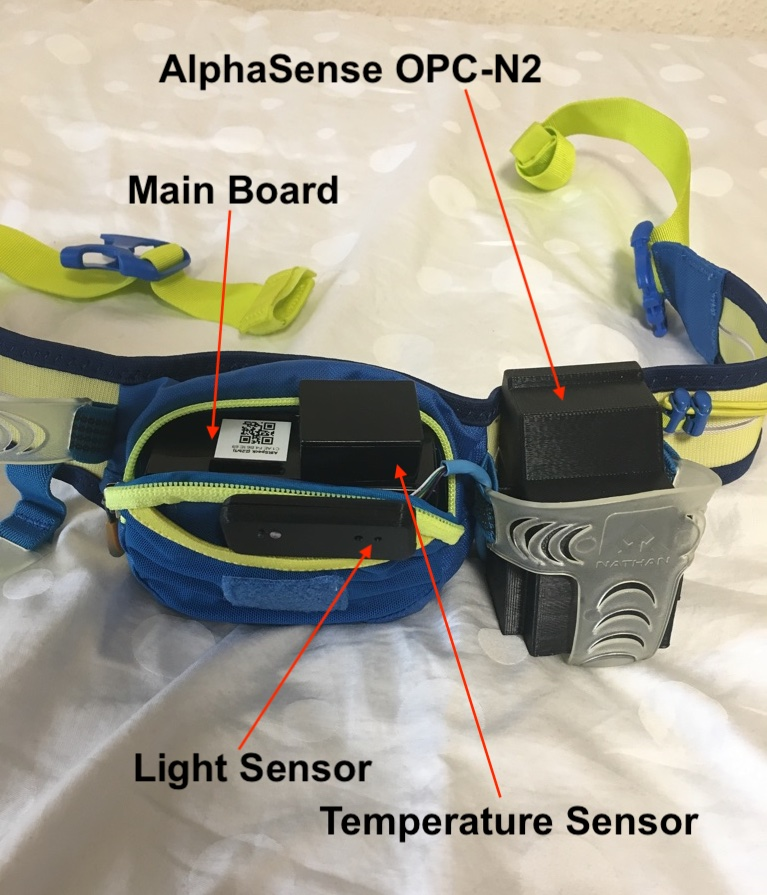
\includegraphics[width=\columnwidth]{airspeck.jpeg} 
  \caption{This picture presents the AirSpeck mobile exposure monitor along with the layout of all the sensors attached to a running belt.}
  \label{fig:airspeck}
\end{figure}


\subsection*{Alphasense Optical Particle Counter}

The data gathered via the Alphasense OPC-N2 \cite{opc} represents the main subject of interest in this project. Size-resolved particulate matter counts are measured in real time, with the latest version of the sensor sampling the environment every 10 seconds. The sensor detects particulates in the range from 0.38 to 17 microns and separates them in 16 different ranges depending on their size \cite{airspeck}. Each range is referred to as a bin, and every bin has a particulate count measurement for the given sampling period. The OPC uses a laser beam and measures the light scattered by individual particulates to determine particulate sizes and counts. PM1, PM2.5, and PM10 measured in $ \mu g /m^3 $ are calculated from the number concentrations detected, assuming negligible contribution from particulates of size less than the lower limit of 0.38 microns.


\subsection*{Temperature Sensor}

A Sensirion SHT-75 temperature and humidity sensor \cite{sensirion} is included on the AirSpeck printed circuit board (PCB) to enable temperature and humidity monitoring without the need to connect to external sensors. The sensor is contained in a waterproof (sintered metal) enclosure \cite{airspeck} and it is placed to protrude outside the enclosure, so that an accurate reading of the temperature and humidity values in the ambient air is ensured.


\subsection*{Communication}

The AirSpeck device has a built-in Bluetooth Low Energy (BLE) radio which communicates with a custom Android application on the mobile device, utilised for receiving and labelling the the sensor readings with time and location (GPS) information. The sensor readings are saved locally in CSV files and they are also forwarded to a remote server for analysis either via cellular network or WiFi.

\section{Urban Environments}
\label{sec:urban-environments}

As far as urban environments detection is concerned, three different urban environments were taken into account in \cite{rome2017} in terms of traffic intensities, as mentioned in section \ref{sec:literature-review}. However, taking only three different categories would not be sufficient to define more complex urban environments with varying traffic vehicular density. For instance, there are certain parts of streets such as bus stops or crossroads which are crowded at peak times of a regular workday, but moderately transited or almost empty during weekends. Another example could include streets edged by two crossroads with one end being crowded at a certain point and the other one being empty. In such situations, smooth transitions between urban environments are most likely to happen in areas approaching the ends of the road in question. In consequence, two additional environment types have been introduced in the current project as transitional urban environments, with the purpose of defining and exploring more accurately such areas with variable traffic intensity. Therefore, the five different urban environments used in this project are the following:

\begin{itemize}
\item Low Vehicular Traffic Density - they are referred to areas with low or non-existent vehicular traffic density, such as park paths, pedestrian zones or quiet roads. One example that was constantly scanned with the purpose of studying personal exposure to different urban environments is the North Meadow Walk in the Meadows Park in Edinburgh, also highlighted in Figure \ref{fig:december_route}.

\item Low to Medium Vehicular Traffic Density - they are referred to transition traffic environments outlined by roads accessible to both pedestrians and vehicles, but with variable traffic intensity at different times of the day such as the middle of Melville Drive around Meadows, also highlighted in Figure \ref{fig:december_route}.

\item Medium Vehicular Traffic Density - they represent areas with medium vehicular traffic density. Relevant examples of such environments include South Clerk Street or Nicholson Street in Edinburgh.

\item Medium to High Vehicular Traffic Density - they are outlined by transition urban environments with variable vehicular traffic density at different times of the day. For instance, a portion of a street might have medium traffic intensity at midday, but higher intensity at peak times such as at approximately 17:30, when most people commute from work. Examples of such urban environments include crossroads between medium traffic streets such as Nicholson Street and West Richmond Street or South Clerk Street and Hope Park Terrace in Edinburgh. 

\item High Vehicular Traffic Density - they represent crowded areas with intense vehicular traffic density during the entire day on average. They are located especially in the city centre and they mostly exist around crowded junctions such as Tollcross or the cross-roads between Princes Street and Telford Road in the West End, as well as crowded bus stops.
\end{itemize}
\label{list:urban-environments}

\section{Personal Exposure with Modes of Transport}

In order to study personal exposure in all cases, six different exposure situations corresponding to six different modes of transport used have been taken into consideration during the data collection process:

\begin{itemize}

\item Pedestrian Data - this represents sensor readings gathered from subjects wearing the AirSpeck device while walking around key areas in Edinburgh, described more thoroughly in \ref{sec:data-collection}.

\item Car - air quality data was collected by Mark Miller (a member of the Centre for Speckled Computing) with the AirSpeck while commuting to work by car in Edinburgh. More details about the routes are presented in \ref{sec:data-collection}.

\item Train - data was also gathered while travelling by train on different routes (From Edinburgh to London and Manchester respectively).

\item Bicycle - bicycle data is composed of two different datasets. One represents data that was collected during the summer of 2015 by Aart Meijer \cite{Meijer2015}, an MSc student while commuting to university by bicycle. Another dataset was gathered in February, during the snow storm. More details regarding the paths are emphasised in \ref{sec:data-collection}.

\item Bus - data was also collected while travelling by bus on different routes around Edinburgh which will be further detailed in \ref{sec:data-collection}. One of the bus routes on which scanning was performed is shown in Figure \ref{fig:bus_route}.

\item Subway (in London) - a small amount of sensor readings were gathered while travelling by subway in London. However, the ambient air scanning was performed during only one trip and hence, this dataset contains few inputs.
\end{itemize}

\chapter{Methodology}

\section{Data Collection Process}
\label{sec:data-collection}

To begin with, the Mobile Exposure Monitor transmits sensor readings to the Android device through the Airspeck app, via Bluetooth Low Energy. Values obtained from OPC measurements are sent every 10 seconds along with GPS coordinates. This ensures an effective spatial representation of the created datasets especially when data is collected at walking speed.

\subsection{Training Dataset Creation}
\label{subsec:training-dataset}

During the project development, an annotated dataset with modes of transport used at each point was created for data analysis. Each data point contains information about the temperature, humidity, GPS coordinates and accuracy, along with PM1, PM2.5, PM10 values and particulate matter counts split into 16 bins. Most of the data was collected in the first semester, more exactly during November and December 2017. First data collection was performed during a train journey from Edinburgh to Manchester, on a route between several train stations for one hour.

Moreover, a major phase of data collection involving the analysis of different types of urban environments occurred between the 3rd and the 8th of December 2017. More precisely, data capturing particulate matter counts had been collected using the MEM, by walking on a fixed route around the Meadows Park in Edinburgh, based on a daily schedule for a week (Figure \ref{fig:december_route}). The route was scanned twice a day, both during lunch time between 13:00 and 14:00 and in the evening between 17:30 and 18:30, so that the same path would be examined at different times of the day involving different traffic intensities.

\begin{figure}[h]
  \center
  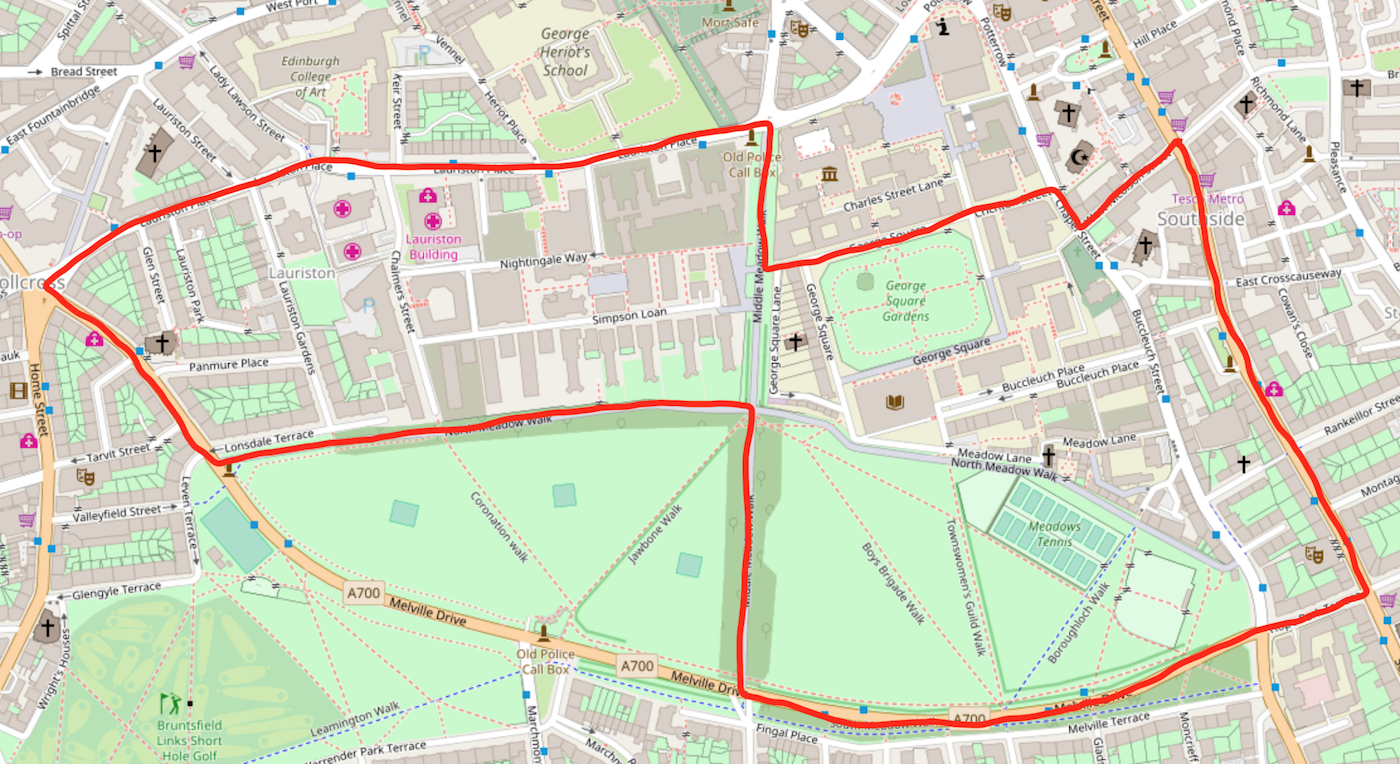
\includegraphics[width=\columnwidth]{december_route.png} 
  \caption{This map of Meadows region emphasises the route that was scanned while walking in December 2017 based on the schedule mentioned.}
  \label{fig:december_route}
\end{figure}

More data gathered and annotated with the purpose of studying personal exposure with different modes of transport has been obtained from Mark Miller who commuted to work by car and wore the device for two consecutive days. He also used the sensors on a train journey to London and around the city centre, involving bus and subway transport. Hence, such a data addition helped balance the categories in the final dataset representing the modes of transport used.

Additional data was collected on bus journeys several times. Firstly, a similar route as the one scanned by Mark Miller (Figure \ref{fig:bus_route}) was taken into account in order to test the types of environment encountered on the route and to balance the final training dataset with the addition of new bus tagged data points. Then, a second bus route between St Andrews Square in Edinburgh and Queensferry was taken into account for scanning. The latter data collection session involved the gathering of both pedestrian and bus labelled inputs and a part of these data points were included in the validation sets described in subsection \ref{subsec:test-data-collection}.

\begin{figure}[h!]
  \center
  \includegraphics[width=\columnwidth]{bus_route.png} 
  \caption{This map emphasises the route that was scanned while taking the bus several times from Waverley station towards Princes Street, George Street and Telford Road.}
  \label{fig:bus_route}
\end{figure}

Furthermore, Aart Meijer, an MSc student whose honours project involved air quality prediction using wearable sensors on cyclists \cite{Meijer2015} collected data on a fixed route around Meadows when he was commuting to university every day by bicycle. A part of the dataset containing approximately 1000 data points has been extracted and compared in \ref{subsec:different-weather} to a new set of data points collected in the evening of the 26th of February 2018 (Figure \ref{fig:february-bike}), during the beginning of the snow storm, in order to analyse how different weather conditions affect sensor readings of particulate matter related information.

\begin{figure}[h!]
  \center
  \includegraphics[width=\columnwidth]{bike_feb.png} 
  \caption{This map emphasises the route that was scanned while taking the bicycle on the 26th of February 2018, during the beginning of the snow storm.}
  \label{fig:february-bike}
\end{figure}

\subsection{Test Data Collection}
\label{subsec:test-data-collection}

Apart from data gathered from different urban environments and by using different modes of transport as described in the previous subsection (\ref{subsec:training-dataset}), additional data has been collected and labelled by other users of the AirSpeck device with the purpose of further validating the classification methods created. The classification results for the validation dataset are thoroughly described in \ref{subsec:results-urban-env-use}.

As previously mentioned in \ref{subsec:training-dataset}, a part of the data points gathered along the bus route between St Andrews Square and Queensferry, Edinburgh, was used only for validation, along with pedestrian tagged inputs that were collected during the trip between bus stations on Princes Street and in Queensferry. Moreover, the trip also included a 12 minute bus journey from Nicholson Street to Princes Street, which was entirely used for validation. The final validation dataset created during this data collection session consists of 501 data points. In order to avoid any possible confusions in references to the validation sets, this dataset will be referred to as \textit{bus\_queensferry\_data}.

Moreover, walking data was collected on the 28th of February by a different subject during the night around the Meadows Park and Nicholson Street in Edinburgh. The dataset created after this gathering session has a total number of 640 data points and all the inputs gathered were used for validation. In future experiments regarding modes of transport classification, this dataset will be referred to as \textit{night\_walk\_data}.

Furthermore, new inputs were collected for validation on a train journey to London by a different subject for about three hours on the 15th of March 2018. A percentage of 25\% of the data points were included in the training dataset with the purpose of balancing the distribution of the labelled inputs by adding more train tagged points. The rest of the data gathered consisting of 600 inputs was used entirely for validation. In future, this dataset will be referenced as \textit{train\_london\_march}.

A separate set of 1278 bike tagged inputs that were collected by Aart Meijer during the summer of 2015 was taken only for validation. The route chosen for this data gathering session is highlighted in Figure \ref{fig:bike-validation-route}. For further reference, this dataset will be nicknamed as \textit{bike\_summer\_route}.

\begin{figure}[h!]
  \center
  \includegraphics[width=\columnwidth]{bike_validation_route.png} 
  \caption{This map emphasises one of the routes that was taken by Aart Meijer during the summer of 2015. The data collected from this scanning session was used entirely for validation purposes.}
  \label{fig:bike-validation-route}
\end{figure}

\section{Data Analysis}
\label{sec:data-analysis}

\subsection{Raw Data Information}

The entire training dataset contains initially a total of 6423 data points. However, there exist points that have missing information related to important attributes such as null temperature and humidity values or null particulate matter counts over the entire series of 16 bins. Thus, these outliers have been removed before proceeding to any experiments as described in subsection \ref{subsec:outlier-removal} and hence, the final, sanitized dataset contains 5409 data points. Figure \ref{fig:distribution} shows the distribution of the training dataset in terms of the labels representing the modes of transport used. As it could be observed, the distribution of inputs over the \textit{on foot}, \textit{train}, \textit{bike} and \textit{bus} labels is balanced as the training dataset contains roughly over 1100 inputs of each type.

\begin{figure}[h!]
  \center
  \includegraphics[width=\columnwidth]{distribution.pdf}
  \caption{This histogram presents the distribution of the data points in terms of the modes of transport labels.}
  \label{fig:distribution}
\end{figure}


\subsection{Outliers in Sensor Readings}
\label{subsec:outlier-removal}

\subsubsection*{Temperature and Humidity Outliers}

Data collected via the AirSpeck devices was not always fully accurate and sometimes data errors were created. For instance, either null or unrealistically high values of the temperature and humidity were sometimes registered at the beginning of data collection sessions after the sensor had been initially started. Figure \ref{fig:outliers} presents the values of the temperature expressed in Celsius degrees, along with the values of the humidity across the training dataset. In the case of the values of temperature data, the lower and upper thresholds were set at -15 and +35 degrees respectively (considering that average temperature in the UK did not exceed these values during data collection). Furthermore, in the case of humidity data, all outliers registering null values were removed.

\begin{figure}[h!]
  \center
  \includegraphics[width=\columnwidth]{outliers.pdf}
  \caption{This set of scatter plots represents the raw values of temperature and humidity data across the entire training dataset with the purpose of highlighting the outliers. The red horizontal lines represent the thresholds that were set to remove the outliers in the data.}
  \label{fig:outliers}
\end{figure}

\subsubsection*{Bin Counts Outliers}

Moreover, sometimes values of particulate matter related data (PM values and bin counts) that were higher than the average or null values were registered by the sensors. Figure \ref{fig:outliers-bins} emphasizes the outliers in the values of the first bin count, as well as the total sum of bin count values for each input. As first bin count had the most dominant values across the training dataset, it has been taken into consideration for the outliers removal procedure along with the total sum of particulate matter counts for each data point.

As it could be observed in the top right scatter plot of Figure \ref{fig:outliers-bins}, the high values of the first outliers for the total sum of bin counts scaled the diagram such that the difference between points with values between 0 and 20000 became unnoticeable. Thus, the first upper threshold for the points representing the sum of particulate matter counts was set at 15000. After removing those outliers, a second threshold was set at 12000 (the bottom left scatter plot), as the large majority of points were placed before that upper bound. In the final step, a final lower threshold was set at 0, such that erroneous data representing points that did not register any bin readings would be removed from the training dataset.

\begin{figure}[h!]
  \center
  \includegraphics[width=\columnwidth]{outliers_bins.pdf}
  \caption{This set of scatter plots represents the raw values of first bin count along with the total sum of particulate matter counts for each data point across the entire training dataset with the purpose of highlighting the outliers. The red horizontal lines represent the thresholds that were set to remove the outliers in the data.}
  \label{fig:outliers-bins}
\end{figure}


\subsection{Mean of Bin Counts}
\label{subsec:bin-count-means}

First, all particulate matter counts have been taken into consideration for analysis in order to visualise the mean values for each bin count over the entire final dataset. Figure \ref{fig:mean_bins_all} shows the distribution of the means of the values for all bin counts over the entire dataset. As it could be observed, bin 0 has the highest values and hence, the distribution of the particulate matter counts is dominated by particulates in bin 0 (range of particulates from 0.38 to 0.52 microns), followed by bins 1 and 2. Therefore, the initial data analysis and visualisation were emphasised mostly on first three bin counts.

\begin{figure}[h!]
  \center
  \includegraphics[width=\columnwidth]{mean_bins_all.pdf}
  \caption{This diagram presents the mean values of all bin counts over the entire final dataset. The histogram on the left presents the raw values on the bin counts, while the one on the right presents the normalised distribution of particulate matter counts.}
  \label{fig:mean_bins_all}
\end{figure}


\subsection{Bin Count Means on Different Weather Conditions}
\label{subsec:different-weather}

Raw data is stored in CSV format and analysis is performed using Python 3.6 and Jupyter Notebooks. In order to check how the weather conditions affect the bin counts, the mean count values of all particulates in the size-resolved bins from 0 to 15 have been calculated for two different datasets collected while using a bicycle on similar routes, but at different times and on different weather conditions. The first dataset was collected by Aart Meijer during the summer of 2015, while the second one was collected on the 26th of February 2018, during the snow storm. Figure \ref{fig:bins_weather} displays the distribution of the bin counts for different weather conditions as previously mentioned. The means of the bin counts have been normalised as described in \ref{subsec:bin-count-normalisation} in order to visualise how the pattern, namely the percentage of each bin value is affected by weather changes.

\begin{figure}[h!]
  \center
  \includegraphics[width=\columnwidth]{bins_weather.pdf} 
  \caption{This set of diagrams represents patterns formed by the distribution of the bin counts expressed in percentages for different weather conditions when a bicycle was the mean of transport used.}
  \label{fig:bins_weather}
\end{figure}

As it could be observed, the percentage of bin 0 decreased during winter while the average percentages of the other bins increased compared to the values obtained during summer. However, similarities in the patterns could be observed as the order of the percentage values for all bin counts is the same.

\subsection{Time Series Analysis of PM Data}

Time series analysis has been performed on the dataset obtained when walking around Meadows area (Figure \ref{fig:december_route}) in order to study the variance of the particulate matter counts in time while changing urban environments. First the dataset has been sorted in ascending order by the time of the day and it has been split in two halves. The first half contains the data collected at lunch time, while the second one consists of data gathered in the evening.

Same analysis has also been performed on the dataset from the journey to and around London in order to analyse how the particulate matter values change in time while switching from a mode of transport to another.

As to the counts of particulate matter, bin 0 has the highest variance, followed by the next two bins, so the first three bins have been taken into consideration for this analysis. Moreover, exponential moving average (EMA), which is implemented in the scikit-learn Python library \cite{scikit-learn}, has been used for visualisation of bin counts (only first three bins as they are the most prominent ones), as well as PM1, PM2.5, and PM10 values respectively in order to ease any transitional event detection (either change of urban environment or mode of transport) by analysing the means of the attributes at each point. Figures \ref{fig:time_series_london} and \ref{fig:time_series_meadows} present the time series analysis of bin counts and PM values for the London journey and Meadows datasets respectively. Moreover, for the London journey dataset, the normalised bin counts have also been taken into consideration in order to discover whether normalisation would ease the detection of modes of transport for the time series analysis. The vertical dashed lines represent the moment when the use of one mean of transport ended during data collection and a new one began until the occurrence of a new line.

\begin{figure}[h!]
  \center
  \includegraphics[width=\columnwidth]{time_series_london.pdf} 
  \caption{This set of diagrams represents the time series analysis of the first three bin counts and PM values for the dataset collected on the journey to London. The Exponential Moving Average is used to express the mean value at each point in time.}
  \label{fig:time_series_london}
\end{figure}

As described in \ref{subsec:bin-count-means}, the first 3 bin counts are the most dominant ones, thus these values were used in the time series analysis and visualisation of particulate matter counts. The first diagram of Figure \ref{fig:time_series_london} presents the exponential moving average of the raw values of the bin counts over time. There could be observed several pollution spikes in the absolute value of bin 0, however no detectable pattern emphasising visible changes of the counts in the event of switching means of transport could be seen.

The next diagram displays the normalised values of the bin counts. In this case, the results have improved, as the percentage level differs visibly form a mean of transport to another, especially for the values of bin 0.

As it could be observed in the third diagram of Figure \ref{fig:time_series_london}, the PM10 values are the most dominant ones across the entire journey. There are pollution spikes from time to time, however, the event of change of a mean of transport is not visually detectable and neither a detectable pattern exists nor a visible difference in the absolute PM values between different means of transport.

\begin{figure}[h!]
  \center
  \includegraphics[width=\columnwidth]{time_series_meadows.pdf} 
  \caption{This set of diagrams represents the time series analysis of the first three bin counts and PM values for the dataset collected while walking in Meadows. The Exponential Moving Average is used to express the mean value at each point in time.}
  \label{fig:time_series_meadows}
\end{figure}

As it could be observed in Figure \ref{fig:time_series_meadows}, there are more frequent spikes in the evening dataset than in midday, meaning that traffic intensity was on average higher at that time of the day. Moreover, the bin values time series diagrams show longer time intervals when the values are high, after which they suddenly decrease and stay at a certain level both in the evening and during midday. For instance, between 17:17:00 and 17:22:00, the average values of bin 0 are much higher than the values between 17:22:00 and 17:37:00. After that point, they begin to slowly increase again, which suggest that a change in the urban environment is occurring. As to the values of PM1, PM2.5 and PM10, the latter has the most dominant values, however no detectable change of the pattern in time could be observed, especially in the dataset containing data collected during midday, where most of the data points present values between 0 and 20 with a spike at about 13:07:00.

\subsection{Pattern Comparison for Different Modes of Transport}

The relative values between all 16 bin counts have also been taken into consideration. Thus, the means for all bin counts corresponding to each mode of transport in particular have been calculated over the entire final dataset and plotted in order to observe any differences in the pattern between two or more modes of transport. Moreover, the same analysis has been performed after applying the bin counts normalisation explained in \ref{subsec:bin-count-normalisation}, in order to visualise the percentage of each bin count that affects personal exposure with each mode of transport (Figure \ref{fig:norm-bins}).

\begin{figure}[h!]
  \center
  \includegraphics[width=\columnwidth]{norm_bins.pdf} 
  \caption{This set of diagrams represents patterns formed by the distribution of the bin counts expressed in percentages for each mode of transport.}
  \label{fig:norm-bins}
\end{figure}

As it could be observed in Figure \ref{fig:norm-bins}, after normalising the values of the particulate matter counts by using the method described in \ref{subsec:bin-count-normalisation}, the patterns between specific modes of transport are visibly distinguishable. For instance, bins 4 and 5 have much smaller values in the case of the car data compared to walking and bicycle datasets. Moreover, bins 7, 8 and 9 have higher values in the case of the bus data compared to any other mean of transport.

\subsection{Spatial Analysis of PM Related Data}

As GPS information is made available by the Android application that collects readings of sensors, a spatial analysis has also been performed on all datasets in order to ease visualisation of urban environment clusters, as well as modes of transport classification predictions performed by the models. The visualisation is performed through a data visualization tool described thoroughly in \ref{sec:data-visualization-tool}. The tool consists of a web interface containing a map which plots the predictions of the data points, as well as a menu allowing the user to tweak custom classification models by choosing between different classification methods and attributes. Moreover, GPS data was used for a more generic approach of detecting urban environments, which is thoroughly described in \ref{subsec:generic-clustering}. A thorough analysis of spatial results obtained in regard to detection of different urban environments is presented in section \ref{sec:urban-environments-results}.


\section{Unsupervised Learning for Urban Environments Detection}

This section emphasises on the methodology performed for detection of different urban environments based on data analysis results explained in section \ref{sec:data-analysis}. The approach is done using unsupervised machine learning technique on several groups of attributes retrieved from sensor readings of the AirSpeck device.

\subsection{K-means Clustering on Particulate Matter Data}
\label{subsec:k-means-methodology}

As a first version of the method, a K-means clustering algorithm is proposed as an approach for automatically detecting different urban environment types based on the distribution of particulate matter values, as well as particulate matter counts. In this way, the values that have a continuous pattern obtained during a certain time interval (Figure \ref{fig:time_series_meadows}) would be clustered in the same group. Particulate matter counts are firstly used as clustering attributes and spatial results obtained are analysed thoroughly in subsection \ref{subsec:k-means-straight-results}.

\subsection{Generalising Clustering Approach by Preserving Locality}
\label{subsec:generic-clustering}

There might be cases in which only the absolute values and counts of particulate matter would not be sufficient for a robust clustering of urban environments. As it could be seen in Figure \ref{fig:time_series_meadows}, there is a significant number of individual spikes in both the PM values and bin counts  from time to time, which would lead to a misclassification of the specific data points. Therefore, in order to generalise the environment type detection, a new approach is proposed with the aim of addressing these edge cases of misclassified points and preserving the same urban environment in a certain area. 

\subsubsection*{Description of Methodology involving Locality Preservation}

In a similar project involving urban environments detection in Edinburgh, \cite{Kotsev2015} proposes a solution in which K-means clustering is applied twice in a row. First, location-based clustering is performed based on the coordinates of the data points and hence, all points within close proximity of each other will be aggregated. The next step involves calculating the means of the attributes for each location cluster. Then, the new means are further clustered into 5 new clusters corresponding to the different urban environments specified in Section \ref{list:urban-environments}. In this way, the classification would be more continuous, as location groups created after the first clustering would be categorised in the same urban environment. Hence, locality preservation would be applied and  the visual representation of an urban environment would be constant in a larger area. Figure \ref{fig:clustering-twice} presents the pipeline of the unsupervised clustering method performed on the data points and Algorithm \ref{alg:k-means-locality} outlines the pseudo-code utilised.

\begin{figure}[h!]
  \center
  \includegraphics[width=\columnwidth]{clustering-twice.pdf}
  \caption{This diagram shows the pipeline of the unsupervised learning method for urban environments detection, applied twice on the dataset.}
  \label{fig:clustering-twice}
\end{figure}

\begin{algorithm}[h!]
 \KwData{input data points from the environment in CSV format}
 \KwResult{data points with corresponding urban environment labels}
 initialization\;
 set \texttt{numberOfLocationClusters}\;
 set \texttt{attributes} to perform clustering on\;
 \tcp{Label the points with corresponding location clusters}
 \texttt{clusteredPoints} $ \leftarrow $ \texttt{KMeans}(coordinates of data points)\;
 calculate means of attributes for all points in each location cluster\;
 environmentClusters $\leftarrow$ \texttt{KMeans}(mean attributes of \texttt{clusteredPoints})\;
 \For{\texttt{cluster} in \texttt{clusteredPoints}}{
   apply the environment label to each point in \texttt{cluster}
 }
 \caption{Pseudo-code of methodology used for urban environments clustering.}
 \label{alg:k-means-locality}
\end{algorithm}

In his project, \cite{Kotsev2015} utilises only the values of bin 0 for the urban environments detection as it represents the most dominant values among all 16 bin counts. However, relying on only one attribute among the 16 bin counts would reduce the information provided from the sensors significantly and hence, misleading results would be produced in certain cases. Thus, experiments utilising all 16 bin counts and PM values respectively are performed separately and obtained results are compared with each other in \ref{subsec:locality-preservation-results}.

\subsubsection*{Decision on the Optimal Number of Location Clusters}

With the latest firmware installed on the AirSpeck device, the sensors collect air quality related information at a rate of one input every 10 seconds. Moreover, in his thesis, \cite{Kotsev2015} uses 50 location clusters on a dataset of around 1846 inputs, so he was sampling the area by using approximately 36 data points per location cluster. However, the firmware installed in the OPC device at that point was registering sensor readings every second, namely one input per second was registered and hence, the density of points in a location was higher ten times higher. Hence,  in the current case regarding the experiments carried out at walking speed around the Meadows route, each area was sampled by using around 15 data points per location cluster instead, because the same route had been crossed for 5 consecutive days during the data collection session. Therefore, at an average walking speed of 1.4 m/s, a journey would be sampled in smaller parts of around 15 metres length each.

\section{Supervised Learning for Modes of Transport Classification}

This section is concerned about the methodology applied for the classification of different modes of transport by using supervised machine learning technique on annotated datasets, the label of each data point representing the mode of transport used at a certain moment.

\subsection{Comparison of Models Performance}

First, several basic models have been trained using the absolute values of the particulate matter counts, as well as the PM1, PM2.5, PM10 values of several datasets containing balanced data points of two or more modes of transport. Moreover, temperature and humidity have been added to the training process in order to visualise how the change of these two attributes in time affects classification accuracy on the validation sets. The models used include logistic regression classifiers (LRC), support vector machine classifiers (SVC), k-nearest neighbours (KNN), random forest classifiers (RFC) and multilayer perceptron classifiers (MLPC). All classification methods previously mentioned are implemented using scikit-learn Python library.

Training of models and classification accuracy score calculations have been performed by using K-Fold cross validation with 5 folds, so that the dataset would be split in 5 equally-sized sets, one of them representing the validation set and the other four being used for training each model. Moreover, the validation datasets that have been collected by other users of the AirSpeck have been used for testing of the models and the accuracy scores obtained have been compared. Then, the top three best performing models have been taken into consideration for further experiments involving model tweaking and data processing in order to increase the overall classification accuracy both over the entire dataset using K-Fold cross validation and the validation sets.

\subsection{Normalisation of Bin Counts}
\label{subsec:bin-count-normalisation}

Absolute values for the particulate matter counts when all 16 bins are taken into consideration differ significantly in different weather conditions or different urban environments. Hence, only taking the absolute values of the particulate matter counts into consideration in the training phase would produce over-fitting of the classification model on the training dataset.

One first approach taken into consideration in order to address this issue was to normalise the bin counts by dividing each of the 16 counts by the total sum of the counts for each data point. Thus, the newly normalised attributes would emphasise the percentage that each particulate matter count would affect personal exposure to individuals when using a certain mode of transport in general.

\subsection{Usage of Urban Environments}

As an attempt to make the classification even more independent of the environment and thus, more generic and accurate for validation sets highlighting edge cases, the results obtained from the urban environments detection method have been used as additional attributes in the model training process for modes of transport classification. Figure \ref{fig:urban-environments-classification-model} displays the final data processing pipeline applied prior to the training phase on the dataset.

\begin{figure}[h!]
  \center
  \includegraphics[width=\columnwidth]{urban-environments-classification-model.pdf}
  \caption{This diagram presents the data processing pipeline which is performed prior to model training for modes of transport classification.}
  \label{fig:urban-environments-classification-model}
\end{figure}

\subsection{Mixed Model Methodology}
\label{subsec:mixed-model-methodology}

As an attempt to improve the classification of modes of transport accuracy and make use of as many attributes available from the OPC as possible, a mixed model containing several classifiers trained on different attributes is proposed. A similar approach, called co-training is used by \cite{Radu2014}, where they present a semi-supervised model for indoor-outdoor detection using smart phones. In order to implement the proposed model, a selection of attributes in terms of their importance should be performed first, followed by a split of the features across multiple classifiers which would be further fitted on the training dataset.


\subsubsection{Feature Selection}
\label{subsubsec:feat-selection}

In order to train the model as accurately as possible and obtain a precise confidence level when deciding on the final predicted labels, the attributes were split in terms of their importance in the classification procedure and distributed along the classifiers. Feature selection and ranking was made in terms of the importance of attributes in the classification problem. The random forest classifier that was used in the classification problem was also utilised for ranking the attributes in terms of their importance (Table \ref{table:attr-rank}).

\begin{table}[h!]
\centering
 \begin{tabular}{||c | c | c | c | c | c||} 
 \hline
 Rank & Attribute \\ [0.5ex] 
 \hline\hline
 1 & total bin counts \\ 
 \hline
 2 &  temperature \\
 \hline
 3 &  environment type \\
  \hline
 4 &  humidity \\
  \hline
 5 &  bin 0 \\
  \hline
 6 &  bin 3 \\
  \hline
 7 &  bin 7 \\
 \hline
 8 & bin 5 \\
  \hline
 9 &  bin 6 \\ 
  \hline
 10 &  bin 4 \\
 \hline
 
\end{tabular}
\caption{This table shows the ranking of the importance of each attribute in the classification of modes of transport problem for top ten attributes. The rankings have been obtained by fitting a random forest classifier on the training dataset.}
\label{table:attr-rank}
\end{table}


\subsubsection{Model Architecture}

After ranking the attributes based on their importance level obtained from the random forest classifier, they were split in such a way to obtain a balanced distribution of attributes in terms of their ranking across two different random forest classifiers. Figure \ref{fig:mixed_model_feature_distribution} presents the architecture of the mixed model along with the distribution of the input attributes based on the importance ranks obtained and shown in \ref{subsubsec:feat-selection}.

\begin{figure}[h!]
  \center
  \includegraphics[width=\columnwidth]{mixed_model_feature_distribution.pdf}
  \caption{This diagram presents methodology for the mixed model used to for validating new inputs after fitting on the training dataset.}
  \label{fig:mixed_model_feature_distribution}
\end{figure}

After dividing the features in two groups, two random forest classifiers are created and fitted on the groups of attributes separately. Next, the probabilities corresponding to the mean of transport labels for validation and test data are predicted using the fitted classifiers. The final confidence value for each label represents the mean of the probabilities obtained for each mean of transport category across the classifiers. Then, the label with the highest confidence value is taken as the final one for each input.


\chapter{Implementation}

\section{Data Visualization Tool}
\label{sec:data-visualization-tool}

This chapter focuses on the data visualization tool which has been implemented with the purpose of easing spatial visualization of results obtained after performing machine learning experiments with regards to urban environments detection and classification of modes of transport. Data is visualized with the help of GPS information provided by the mobile device through the AirSpeck Android app during data collection. Figure \ref{fig:vis-tool} describes briefly the main structure of the data visualization tool which will be further explained in the next three subsections.

\begin{figure}[h!]
  \center
  \includegraphics[width=\columnwidth]{vis-tool.pdf}
  \caption{This diagram presents briefly the main structure of the data visualization tool built with the purpose of easing spatial visualisation of results obtained after performing machine learning experiments.}
  \label{fig:vis-tool}
\end{figure}


\subsection{Database}
\label{subsec:database}

\subsubsection*{Motivation for Database Implementation}

The training data is stored in a database which configured using \texttt{PostgreSQL} \cite{postgres}. The main reason behind using a database system is the extra layer of security provided for the training data. Moreover, PostgreSQL has native support for using SSL connections and hence, connections with the back-end server are encrypted. Therefore, a secured storage of the training data will provide an additional layer of protection against system breaks from external users.

\subsubsection*{Database Structure}

The structure of the database system is shown in Figure \ref{fig:database}. It consists of three tables. Table \texttt{mode\_of\_transport} contains the names and unique identifiers of all labels for the modes of transport. The \texttt{dataset} table contains the ids and names of the datasets that currently exist in the database and whose inputs are stored in one place as training data points. Finally, table \texttt{collected\_data} contains all the data points from all the datasets that have been uploaded by the user. In Figure \ref{fig:database}, \textit{[Airspeck Attributes]} refers to all attributes of the data points that exist in the CSV files created by the AirSpeck Android app during data collection. In addition, the table contains two mandatory foreign keys, one to the \texttt{mode\_of\_transport} table and the other one to the \texttt{dataset} table.

There is no table for urban environments, as the method performed for environment type detection is unsupervised and classification results will always differ based on the training dataset taken in consideration and validation data that is queried. More information about handling urban environment indices is provided in subsection \ref{subsec:back-end}, which presents the back-end structure.

\begin{figure}[h!]
  \center
  \includegraphics[width=\columnwidth]{database.pdf}
  \caption{This diagram presents briefly the main structure of the data visualization tool built with the purpose of easing spatial visualisation of results obtained after performing machine learning experiments.}
  \label{fig:database}
\end{figure}

\subsection{Back-end Server}
\label{subsec:back-end}

A back-end server has been developed as a common part with Vlad Buzatu, a student who works on a different AirSpeck related honours project. Thus, as Figure \ref{fig:vis-tool} also shows, the back-end server functionality is divided in two parts corresponding to two different API's concerned about the two different projects. This section will focus on the implementation of the API of the author (Mihai's API). A setup guide for the API and its dependencies is outlined in section \ref{sec:api-setup}.

\subsubsection*{Motivation for Framework Choice}

The server has been created using Django 2 Framework \cite{django}. The main reason behind choosing Django 2 for back-end development is that it is a high-level framework written in Python 3, which makes it significantly easier to migrate the machine learning models developed in Jupyter Notebooks to the back-end side of the tool. Moreover, it provides efficient and secure connections both to the database which is further described in subsection \ref{subsec:database} and the front-end interface, detailed in subsection \ref{subsec:front-end}.

\subsubsection*{Connection to Database}

Django framework provides full support for PostgreSQL databases and connection is established once the framework first makes a database query. This connection is then kept open and reused in subsequent requests.

Database queries are performed through Django objects that belong to classes called data models \cite{django-queries}, which are custom classes written in Python. In other words, each data model corresponds to a table in the database and the properties of a class represent the fields in the corresponding table. In addition, each data model instance represents an input which is stored in the database table. Furthermore, once the structure of a data model has been modified or a data model has been either created or deleted, the operation is synchronised with the database and applied to the schema through so-called \texttt{migrations} \cite{django-migrations}.

\subsubsection*{Connection to Front-end Interface}

As to the connection of the server to the front-end interface, \texttt{ngrok} \cite{ngrok}, a multi-platform tunnelling software has been used for development, as it establishes secure tunnels from a public endpoint where the back-end server stands to the front-end running locally. 

Moreover, in order to maintain communication between two different endpoints running on different systems, the \texttt{django-cors-headers} \cite{django-cors} library was used with the purpose of handling connection request headers that are required for Cross-Origin Resource Sharing (CORS) \cite{cors}.

Django framework provides an efficient way of handling connection requests through the use of so-called \texttt{views} \cite{django-views}. A view is most generally a function that takes a web request from the front-end interface and returns a web response. In the case of the current project, the response returned from the back-end API will be in \texttt{JSON} format \cite{json} and will be further interpreted by the front-end interface. The current structure consists of 4 different views 4 different requests (Figure \ref{fig:views}).

\begin{figure}[h!]
  \center
  \includegraphics[width=\columnwidth]{views.pdf}
  \caption{This diagram shows the structure of the Django views used for handling web requests and responses.}
  \label{fig:views}
\end{figure}

The urban environments detection view is responsible for applying the clustering methods using the parameters sent from the front-end menu as clustering attributes. The clustering and modes of transport classification menus will be further described in subsection \ref{subsec:front-end}. The modes of transport classification view is handles requests regarding modes of transport classification for datasets specified by the user and returns the labelled data as a response to the interface. The dataset view returns unique identifiers and names of all datasets that exist in the database as a response in JSON format once the interface has finished loading in the web browser. Moreover, the new data upload view contains the back-end functionality of the new data upload tool which is utilised for storing new labelled data points in the database and performing machine learning predictions on unlabelled data.


\subsubsection*{Classifiers Implementation}

The classifiers are initialised in the views related to modes of transport and urban environments respectively and are implemented using \texttt{scikit-learn} \cite{scikit-learn} Python library. The user has the ability to select from a range of classifiers in order to either perform urban environments and modes of transport predictions on new data or test performance of the classification method settings using K-Fold cross validation on a training dataset chosen by the user. Furthermore, the user has the ability to select the number of folds to use while performing cross-validation, so that they can choose the percentage of the training data that would be taken for validation. As to the attributes used for urban environments detection and modes of transport classification, the user has the ability to choose which attributes to use. Moreover, a choice of whether to use bin counts normalisation in the classification methods is provided by the interface. All these settings configured by the user on the interface are sent through requests to the back-end and handled in the views.


\subsection{Front-end Interface}
\label{subsec:front-end}

The front-end side of the visualization tool consists of an interface which sends user requests to the API located in the back-end server and receives back responses containing data with the corresponding modes of transport or urban environments labels based on the classification methods the user chooses to apply. As it runs separately from the back-end, a different server configuration needed to be set up for the front-end to run. During development, the interface was firstly running on a simple Python server using the \texttt{http.server} module from Python 3. However, this solution was throwing errors while testing the new data upload tool, as the server was unable to send POST requests remotely. Therefore, the interface structure was reorganised and configured to run on a Flask server \cite{flask} which has the ability to send both POST and GET requests to the Django back-end server remotely.

The front-end consists of three main parts which are further described in the following paragraphs. The general design of the interface and the navigation menu between the three parts have been developed using the \texttt{Semantic-UI} library \cite{semantic-ui}.

\subsubsection*{Map Interface}

The map interface is the main part where the results are displayed based on the spatial information that the data contains.  The map interface is built using the \texttt{LeafletJS} library \cite{leaflet}. Each data point is represented as a circle with the radius proportional to the total sum of bin counts. Each circle is coloured differently based on the corresponding mode of transport or urban environment that has been attached to each data point in the API response. Figure \ref{fig:map-interface} outlines the map interface which is used to visualise the results obtained based on the GPS information of the input data, after performing classification and clustering tasks from the classifiers interface.

\begin{figure}[h!]
  \includegraphics[width=\textwidth]{map-interface.png}
  \caption{The main interface which implements a map tool used to visualize the results of the classification and clustering tasks based on the GPS information of the input data.}
  \label{fig:map-interface}
\end{figure}

\subsubsection*{Classifiers Menu}

The classifiers menu represents the main interface which offers the user the ability to customise their own classification model, either for the task of modes of transport classification or urban environments detection. Moreover, the user is able to either apply K-Fold cross validation with a custom number of folds on the training dataset and test the classification accuracy or select an entire dataset for validation and predict the corresponding labels based on the chosen classification task. Figure \ref{fig:classifiers-interface} presents the main interface which allows the user to configure the settings for the classification and clustering models and obtain visual results which are made visible on the map interface, as well as accuracy results in the case of modes of transport classification. Section \ref{sec:menu-usage} presents a more detailed utilisation guide for the classifiers menu through which its functionality and flexibility are emphasised.

\begin{figure}[h!]
  \includegraphics[width=\textwidth]{classifiers-interface.png}
  \caption{The main interface which allows the user to configure the classification and clustering models and perform both modes of transport classification and urban environment detection tasks on datasets.}
  \label{fig:classifiers-interface}
\end{figure}

\subsubsection*{New Data Upload Tool}

The new data upload tool is responsible for handling new data that is uploaded by the user in CSV format. The user is able to upload either unlabelled or labelled data with modes of transport tags. In the case of labelled inputs, the new dataset will be stored in the database as training data and the user has the ability to name it for future referencing. On the other hand, if the inputs are unlabelled, the user will be able to decide whether to perform clustering for urban environment detection or classification of modes of transport on the new data points. In the latter case, the CSV file will be uploaded from the classifiers menu and the data will be loaded on the back-end through \texttt{pandas} dataframes \cite{pandas}. Figure \ref{fig:upload-tool} presents the interface of the data upload tool. The first input allows the user to either select a dataset which already exists to add the new data to or create a new one. Then, a file upload input is implemented which allows the user to upload new files containing data points in CSV format. In addition, by pressing on the sidebar icon situated on the left side of the title in this case, the main menu of the data visualisation tool will appear (FIgure \ref{fig:menu}).


\begin{figure}[h!]
  \begin{subfigure}[t]{\textwidth}
    \includegraphics[width=\textwidth]{menu.png}
    \caption{The main menu of the interface which is accessed by pressing on the menu icon situated on the left side of the titles.}
    \label{fig:menu}
  \end{subfigure}
  \hfill
  \begin{subfigure}[t]{\textwidth}
    \includegraphics[width=\textwidth]{upload-tool.png}
    \caption{Data upload tool implemented on the front-end interface which is used to upload new data points in the database and label the inputs to a corresponding dataset.}
    \label{fig:upload-tool}
  \end{subfigure}
  \caption{New data upload tool and the general menu of the interface.}
  \label{fig:upload-tool-and-menu}
\end{figure}


\chapter{Results}

\section{Detection of Urban Environments}
\label{sec:urban-environments-results}

One main set of experiments regarding detection of urban environments has been performed mostly using the dataset created during the one week data collection session around the Meadows in December 2017 (Figure \ref{fig:december_route}). First, the entire dataset was split in two subsets, the former one consisting of all data collected during midday and the latter one containing all inputs gathered in the evening, as described in subsection \ref{subsec:training-dataset}.

\subsection{K-Means Clustering on PM Related Data}
\label{subsec:k-means-straight-results}

As presented in subsection \ref{subsec:k-means-methodology}, an unsupervised learning approach using K-means clustering was taken into account for urban environment detection. At first, clustering was applied directly on the raw values of the bin counts and particulate matter values separately.

Figure \ref{fig:urban_afternoon_bins_no_loc.png} shows a spatial representation of the urban environments obtained on the dataset collected during the evening sessions after applying a K-means classifier on the bin counts directly. As it could be observed, no visible pattern is obtained and the points are randomly clustered based on the values of the bin counts. The majority of the data points are labelled as medium vehicular traffic density areas with medium to high and low to medium traffic intensity area-tagged inputs in between.

\begin{figure}[h!]
  \center
  \includegraphics[width=\columnwidth]{urban_afternoon_bins_no_loc.png}
  \caption{This map presents the urban environments detected on the evening dataset after applying K-means directly on the bin counts of the data points.}
  \label{fig:urban_afternoon_bins_no_loc.png}
\end{figure}


\subsection{Generalisation of Clustering Approach through Locality Preservation}
\label{subsec:locality-preservation-results}

In order to obtain a more solid visual representation of an urban environment in a specific area, locality preservation has been added (method is described in subsection \ref{subsec:generic-clustering}) by using another K-means classifier prior to the urban environments clustering on the coordinates obtained from the spatial information of the data points. Figure \ref{fig:urban_afternoon_bins} shows the new visual representation of the urban environments after applying locality preservation prior to clustering of the bin counts on the evening dataset (same dataset as the one represented in Figure \ref{fig:urban_afternoon_bins_no_loc.png}). In this case, the labelled points visually outline urban environments as parts of the roads contained in the route taken. Further discussion on the obtained environments and a comparison between clustering on PM values against bin counts are presented in subsection \ref{subsec:afternoon-midday-results}.


\subsection{Comparison between Evening and Midday Environments}
\label{subsec:afternoon-midday-results}

This subsection presents an analysis of the results obtained after performing urban environments detection on the midday and evening datasets separately, taking into consideration different sets of attributes.

\subsubsection*{Clustering on Bin Counts}

Figures \ref{fig:urban_afternoon_bins} and \ref{fig:urban_midday_bins} present the urban environments detected based on bin counts clustering for the evening and midday datasets respectively, after applying the generalised classifier using locality preservation.

As it could be observed, the south side of the route is similar in both cases, with the majority of inputs labelled as low and low to medium vehicular traffic density zones. This result might be due to the fact that traffic was not as intense on Melville Drive as in other parts of the route and the road crosses along the border of the Meadows Park. Moreover, the central area between Middle Meadow Walk and North Meadow Walk (two separate alleys crossing the Meadows Park) has been labelled as a low traffic density area in the case of both times of the day, which shows that pollution was always low in the middle of the park during the data collection session.

On the other hand, the classifier detected more polluted areas on the northern side of the route in the case of the evening dataset compared to inputs gathered during midday, namely on Tollcross, Lauriston Place and Teviot Place. This result emphasises the higher pollution during a peak hour (between 17:30 and 18:30) when most people commute from work. In addition, at both times of the day, medium to high and high traffic areas have been detected around crowded bus stations both on Nicholson Street and Lauriston Place. Furthermore, pollution spikes can be visualised around street junctions such as the Tollcross area (crossroads between Earl Grey Street, Home Street and Lauriston Place), Teviot Place and the crossroads between South Clerk Street and Bernard Terrace.


\begin{figure}[h!]
  \center
  \includegraphics[width=\columnwidth]{urban_midday_bins.png}
  \caption{This map presents the urban environments detected on the midday dataset after applying K-means clustering first on the coordinates and then on the bin counts of the data points.}
  \label{fig:urban_midday_bins}
\end{figure}

\begin{figure}[h!]
  \center
  \includegraphics[width=\columnwidth]{urban_afternoon_bins.png}
  \caption{This map presents the urban environments detected on the evening dataset after applying K-means clustering first on the coordinates of the data points and then on the bin counts of the data points.}
  \label{fig:urban_afternoon_bins}
\end{figure}

\subsubsection*{Clustering on PM Values}

In this set of experiments regarding urban environment detection, the PM 1, PM 2.5 and PM 10 values collected on the same route were taken into consideration. Figures \ref{fig:urban_midday_pm} and \ref{fig:urban_afternoon_pm} present the urban environments that were detected for the midday and evening datasets respectively, after applying the generalised classifier based on locality preservation, also mentioned in \ref{subsec:locality-preservation-results}.

In the case of the southern part of the route, the majority of the data points were again tagged as low and low to medium traffic density areas for both times of the day. However, on the left side of the North Meadow Walk there are more data points clustered in the latter category in the evening dataset compared to the one created during midday. This situation outlined similar results to the ones when the bin counts were used for clustering instead. This suggests that in overall, over the 5 days of scanning, that part of the route is more polluted in the evening than at lunch time. Moreover, higher pollution results were registered at the crossroads between Melville Drive and Argyle Place during the evening scanning sessions, as most of the labels in that place were tagged as low to medium traffic intensity areas.

As to the northern part of the route, the results outlined areas that were on average more polluted in the evening than at midday (the crossroads between Nicholson Street and West Nicholson Street, along with Tollcross area). However, some parts such as the upper side of the Middle Meadow Walk and the north-western side of George Square were labelled as high traffic, which in reality are pedestrian alleys. Moreover, the crossroads between Earl Grey Street, Home Street, Lauriston Place and Broughton Street in Tollcross were labelled as low to medium traffic density areas at lunch time and medium traffic intensity areas in the evening, which shows that on average, vehicular traffic density increases at peak times in the evening when most people commute from work.


\begin{figure}[h!]
  \center
  \includegraphics[width=\columnwidth]{urban_midday_pm.png}
  \caption{This map presents the urban environments detected on the midday dataset after applying K-means clustering first on the coordinates and then on the PM values of the data points.}
  \label{fig:urban_midday_pm}
\end{figure}

\begin{figure}[h!]
  \center
  \includegraphics[width=\columnwidth]{urban_afternoon_pm.png}
  \caption{This map presents the urban environments detected on the evening dataset after applying K-means clustering first on the coordinates and then on the PM values of the data points.}
  \label{fig:urban_afternoon_pm}
\end{figure}

\subsubsection*{General Difference of Results at Different Day Times}

From the results obtained regarding urban environment detection at different times of the day, it could be observed that the moment of the day at which the data collection process is performed represents a major factor in a realistic detection of urban environments in key areas of a route. For instance, it has been shown that a certain part of a street, such as a crowded bus station or a junction can be more crowded at peak times (17:30-18:30) than during midday (13:30-14:30) and hence, the pollution levels are much higher, which results in data points tagged as medium and high traffic areas.

The following subsection (\ref{subsec:bin-counts-pm-vals}) outlines the differences in the results obtained when the bin counts were considered for clustering as opposed to the case when the PM values were used instead.

\subsection{Bin Counts Against PM Values Classification}
\label{subsec:bin-counts-pm-vals}

As the results obtained by the unsupervised model after classifying the inputs based on the bin counts and PM values respectively differ significantly, a debate discussing the differences is necessary. 

\subsubsection*{Evening Dataset}

First, it could be observed that in the case of the evening dataset, the bin counts prove to be more sensitive as for the northern side of the route, the classifier detected areas of higher pollution (medium to high traffic areas on Lauriston Place and Broughton Street and high traffic zones around crowded bus stations on Lauriston Place).  In addition, the upper side of Middle Meadow Walk has been classified entirely as a medium to high traffic area when PM values were taken into consideration, in contrast with the case when the bin counts were used and the alley was labelled as a medium traffic intensity area. Moreover, the path crossing along the edge of St. Patrick square (between Nicholson Street and Clerk Street), which is usually a medium traffic street at peak times has been labelled as a low traffic area in the case of the PM values (Figure \ref{fig:south-clerk-afternoon-pm}). In contrast, the same area has been tagged as a medium traffic intensity zone when the clustering model used the bin values as main attributes (Figure \ref{fig:south-clerk-afternoon-bins}).

\begin{figure}[h!]
  \begin{subfigure}[t]{0.5\textwidth}
    \includegraphics[width=\textwidth]{south_clerk_afternoon_pm.png}
    \caption{Urban environments detection when PM values were used for clustering.}
    \label{fig:south-clerk-afternoon-pm}
  \end{subfigure}
  \hfill
  \begin{subfigure}[t]{0.5\textwidth}
    \includegraphics[width=\textwidth]{south_clerk_afternoon_bins.png}
    \caption{Urban environments detection when bin counts were used for clustering .}
    \label{fig:south-clerk-afternoon-bins}
  \end{subfigure}
  \caption{Comparison between results on South Clerk Street when PM values and bin counts were used for clustering on the evening dataset separately.}
  \label{fig:south-clerk-comparison}
\end{figure}


\subsubsection*{Midday Dataset}

In the case of the midday dataset, it could be observed that the bin counts are again more sensitive on the northern side of the route as results representing higher pollution levels have been registered. More precisely, Tollcross junction outlined low to medium traffic intensity areas and Lauriston Place outlined mostly medium to high traffic zones around crowded bus stations when PM values were used for clustering. On the other hand, when bin counts were utilised, higher pollution levels were registered in the same area, namely medium to high traffic area in Tollcross and high traffic zones around crowded bus stations on Lauriston Place. The latter results obtained are closer to a real scenario on average, as Lauriston Place and the crossroads in Tollcross are usually crowded zones.

\subsubsection*{Number of Discontinuities as a Validation Measure}

As it could be observed in Figure \ref{fig:south-clerk-comparison}, a discontinuity in the resulted labels has been obtained in the case of urban environments clustering when PM values were used for the evening dataset. More precisely, a discontinuous transition from a medium to highly polluted environment to a low pollution zone occurred on a main street of the city which is frequently transited by buses. Moreover, considering the sensor reading rate of 10 inputs per second and the walking speed at which data was collected, a transition from an urban environment to another should be smooth and generally all pollution levels should be detected within a certain interval.

In consequence, the number of discontinuities on a certain route has been taken into account as a validation measure for urban environments detection when using different attributes. Table \ref{table:discontinuities-meadows} presents the number of discontinuities occurring on the midday and evening datasets after performing urban environments detection using PM values and bin counts as clustering attributes separately , as well as values of bin 0 alone as proposed by Konstantin Kotsev in \cite{Kotsev2015}after applying location clustering for locality preservation. As it could be observed, the number of discontinuities is significantly higher in the case of PM values. Moreover, in the case when only bin 0 was used for clustering, the number of discontinuities increased for both datasets. Hence, this measure shows that the usage of all bin counts is more reliable and produces more robust results regarding urban environments clustering on pedestrian data.

\begin{table}[h!]
\centering
 \begin{tabular}{||c | c | c | c||} 
 \hline
 Dataset & PM Values & All Bin Counts & Bin 0 \\ [0.5ex] 
 \hline\hline
 Midday Dataset & 6 & 3  & 4 \\ 
 \hline
 Evening Dataset & 6 & 4 & 5 \\
 \hline
\end{tabular}
\caption{This table presents the number of transition discontinuities occurring in the labels of the pedestrian dataset after applying unsupervised learning for urban environments detection.}
\label{table:discontinuities-meadows}
\end{table}

\subsubsection*{Validation of Results Against Live Traffic Data}

Google Traffic is a feature available on Google Maps which displays information regarding traffic conditions in real time. The service works by analysing GPS information such as coordinates and average speed along a section of a road from a large number of mobile phones users. Hence, assuming that low traffic speed implies high vehicular traffic density on a certain route, it was considered that Google Traffic data could represent an accurate validation measure for the results obtained regarding detection urban environments characterised by high traffic intensity using the unsupervised learning method described in \ref{subsec:generic-clustering}. Figure \ref{fig:meadows-google-maps} displays the average vehicular traffic speed on the major roads around the Meadows Park in Edinburgh on a Thursday, at about 17:15 (similar time to the one when the evening data collection sessions were conducted).

\begin{figure}[h!]
  \center
  \includegraphics[width=\columnwidth]{meadows_google_maps.png}
  \caption{This map shows the average traffic speed on the main roads around the Meadows Park in Edinburgh on a Thursday, at about 17:15. The data is made available via the Google Traffic Service which is available on Google Maps.}
  \label{fig:meadows-google-maps}
\end{figure}

As it could be observed on Google Traffic data, average traffic speed is slower on the upper left section of Melville Drive heading towards Tollcross. Moreover, the same section of the road was tagged as a high vehicular traffic density zone on the evening pedestrian dataset when bin counts were selected as clustering attributes. Furthermore, the crossroads between Potterrow and Nicholson Street present slow traffic on Google Traffic data. At the same time, the same area was tagged as a high vehicular traffic density zone by the unsupervised model when bin counts were taken into account for clustering. Hence, high vehicular traffic density areas were discovered via both the unsupervised model when the bin counts were considered as clustering attributes and the Google Traffic service.


\subsection{Urban Environments Detection Applied on Other Modes of Transport}
\label{subsec:urban-envs-on-modes-of-transport}

Apart from the walking data gathered on the route around Meadows Park described in section \ref{sec:data-collection}, the urban environments detection method presented in \ref{subsec:generic-clustering} has been applied on other modes of transport, more exactly on cycling routes and bus journeys.

\subsubsection*{Urban Environments Detection on a Bus Journey}

Urban environments detection has been applied using both PM values and bin counts separately on the return bus journey from St Andrews Square in the city centre to Queensferry bridges. Figure \ref{fig:queensferry-urban-environments} shows the route taken and the data points labelled with their corresponding urban environments after applying clustering using the bin counts and PM values separately.

\begin{figure}[h!]
  \begin{subfigure}[t]{\textwidth}
    \includegraphics[width=\textwidth]{bus_envs_pm.png}
    \caption{Urban environments detection when PM values were used for clustering.}
    \label{fig:queensferry-env-pm}
  \end{subfigure}
  \hfill
  \begin{subfigure}[t]{\textwidth}
    \includegraphics[width=\textwidth]{bus_envs_bins.png}
    \caption{Urban environments detection when bin counts were used for clustering .}
    \label{fig:queensferry-env-bins}
  \end{subfigure}
  \caption{Comparison between results obtained on the Queensferry bus route when PM values and bin counts were used for clustering separately.}
  \label{fig:queensferry-urban-environments}
\end{figure}

As it could be observed, in the case of bin counts usage on the environments detection model, the transitions are smooth and clustering results are closer to a real scenario, as Princes Street and the junction between Princes Street and Queensferry Street are crowded zones that are often transited by buses. Moreover, there is a large number of bus stops on Queensferry Road and thus, corresponding data points were tagged as high traffic areas as the doors were held open at every stop and the traffic congestion created by the buses queueing increased pollution levels significantly and thus, the number of particles in each bin count.


\subsubsection*{Urban Environments Detection on Cycling Routes}

Furthermore, urban environments clustering has also been applied on two datasets corresponding to two different cycling routes (section \ref{sec:data-collection}), one created by Aart Meijer in the summer of 2015 (Figure \ref{fig:meijer-bike-urban-envs}) and the second created by the author on the 26th of February 2018 (Figure \ref{fig:feb-bike-urban-envs}).

\begin{figure}[h!]
  \begin{subfigure}[t]{0.5\textwidth}
    \includegraphics[width=\textwidth]{urban_envs_aart_meijer_pm.png}
    \caption{Urban environments detection using PM values for clustering on Aart Meijer's cycling route over the summer.}
    \label{fig:meijer-bike-urban-envs-pm}
  \end{subfigure}
  \hfill
  \begin{subfigure}[t]{0.5\textwidth}
    \includegraphics[width=\textwidth]{urban_envs_aart_meijer_bins.png}
    \caption{Urban environments detection using bin counts for clustering on Aart Meijer's cycling route over the summer in 2015.}
    \label{fig:meijer-bike-urban-envs-bins}
  \end{subfigure}
  \caption{Urban environments detection on Aart Meijer's cycling route over the summer in 2015}
  \label{fig:meijer-bike-urban-envs}
\end{figure}

\begin{figure}[h!]
  \begin{subfigure}[t]{\textwidth}
    \includegraphics[width=\textwidth]{urban_env_feb_bike_pm.png}
    \caption{Urban environments detection using PM values for clustering on the data collected on the February 2018 cycling route.}
    \label{fig:feb-bike-urban-envs-pm}
  \end{subfigure}
  \hfill
  \begin{subfigure}[t]{\textwidth}
    \includegraphics[width=\textwidth]{urban_env_feb_bike_bins.png}
    \caption{Urban environments detection using bin counts for clustering on the data obtained on the February 2018 cycling route.}
    \label{fig:feb-bike-urban-envs-bins}
  \end{subfigure}
  \caption{Urban environments detection on the data obtained during the February 2018 cycling route.}
  \label{fig:feb-bike-urban-envs}
\end{figure}

As it could be seen, in the case of the February cycling route, the clustering method using bin counts produced again smooth results that are also closer to a real scenario as opposed to the clustering method using PM values. More precisely, the entire zone outlined by Leamington Walk (a cycling path crossing through the park) has been labelled as a low to medium vehicular traffic density area. Moreover, in the case of Aart Meijer's cycling route, Middle Meadow Walk was entirely labelled as a low traffic area with edges tagged as low to medium traffic density zones, while in the case of the PM values, a discontinuity in the transition between urban environments occurred in the same area.


\subsubsection*{Number of Discontinuities}

As to the case of the bus journey to the Queensferry bridges, there are again significantly less transition discontinuities from an environment to another when clustering on bin counts was applied compared to the case in which the PM values were used. Hence, usage of bin counts in the urban environments detection model proves to be again more robust as opposed to the usage of PM values. Furthermore, in the case of Aart Meijer's cycling route, there are less transition discontinuities between urban environments when applying clustering based on the bin counts as opposed to the case when PM values were utilised. On the other hand, the result is different in the case of the cycling route scanned on the 26th of February 2018. This result might occur due to exceptional snowy weather conditions, and hence, the low traffic intensity encountered in that period, which resulted in lower pollution levels detected when bin counts were taken into consideration for clustering. In addition, the hysteresis effect present in the sensor readings cause a delay in particulate matter data scanning in ambient air which leads to certain areas being labelled with misleading environments (e.g. a part of Bruntsfield Place was tagged as a low vehicular traffic density area, straight after the lower portion being clustered as a medium traffic intensity zone). Table \ref{table:discontinuities-bike-bus} presents the number of discontinuities for each dataset obtained when PM values and bin counts were used for the clustering problem separately.


\begin{table}[h!]
\centering
 \begin{tabular}{||c | c | c ||} 
 \hline
 Dataset & PM Values Clustering & Bin Counts Clustering \\ [0.5ex] 
 \hline\hline
 Return Bus Journey to Queensferry & 3 & 0 \\ 
 \hline
 February Cycling Route & 3 & 4 \\
 \hline
 Aart Meijer's Cycling Route & 9 & 2 \\
 \hline
\end{tabular}
\caption{This table presents the number of transition discontinuities occurring in the labels of the pedestrian dataset after applying unsupervised learning for urban environments detection.}
\label{table:discontinuities-bike-bus}
\end{table}


\subsubsection*{Validation of Results Against Live Traffic Data}

As in the case of the model validation on the dataset collected during the evenings around the Meadows Park, a comparison of the obtained results with Google Traffic data was considered in the case of the return bus journey between St Andrews Square and Queensferry as well. Figure \ref{fig:queensferry-google-maps} shows the average traffic speed on the route to Queensferry on a Thursday, at around 17:05.

\begin{figure}[h!]
  \center
  \includegraphics[width=\columnwidth]{queensferry_google_maps.png}
  \caption{This map shows the average traffic speed on the main roads including the route to Queensferry Edinburgh on a Thursday, at about 17:05. The data is made available via the Google Traffic Service which is available on Google Maps.}
  \label{fig:queensferry-google-maps}
\end{figure}

As it could be observed, the section of Queensferry Road edging the crossroads with Maybury Road and Dean Village presents a slow traffic area on Google Traffic data. In addition, the unsupervised model labelled the inputs on the same part of the route as medium to high and high traffic intensity points respectively when bin counts were taken into consideration. Hence, the model was again able to detect a high traffic density environment accurately based on particulate matter counts retrieved from sensor readings of the AirSpeck device. Furthermore, the upper side of Queensferry Road located towards the suburbs of Edinburgh City presents fast traffic on Google Traffic data. At the same time, the inputs located on the same portion of the road were tagged as medium and low to medium vehicular traffic density points by the unsupervised model. This result emphasises the fact that pollution levels start to decrease as traffic becomes more fluid on the road.


\section{Comparison of Personal Exposure with Different Modes of Transport}

This section presents the results obtained after training different models and testing different methods for the classification of modes of transport problem.

\subsection{Classification on absolute values of attributes}
\label{subsec:abs-values-models}

Several pairs of attributes have been used for training different models. First, all 16 particulate matter count bins have been taken into consideration. Then, the number of bin counts taken for training has been reduced to 3, as the first three bins proved to be the most dominant ones. Separately, the PM1, PM2.5 and PM10 values have been taken for training and the mode of transport classification accuracies obtained have been compared with the former case. 

Table \ref{table:abs-values-models} presents the validation accuracies obtained using K-Fold cross validation for each classification method after training the models on the raw attribute values of the entire dataset. As it could be observed, the best performing model was the one implementing a random forest classifier on all bin 16 bin counts. Therefore, for the next experiments involving data processing and model optimisation, the 16 particulate matter counts have been taken into consideration for training and testing.

\begin{table}[h!]
\centering
 \begin{tabular}{||c | c | c | c | c | c||} 
 \hline
 Classification Method & All Bin Counts & First 3 Bin Counts & PM Values \\ [0.5ex] 
 \hline\hline
 SVC & 55.4\% & 54.9\% & 76.6\% \\ 
 \hline
 LRC & 78.6\% & 68.0\% & 66.5\% \\
 \hline
 KNN & 84.6\% & 79.3.0\% & 76.7\% \\ 
 \hline
 \textbf{RFC} & \textbf{87.4}\% & 79.8\% & 78.9\% \\ 
 \hline
  MLPC & 77.2\% & 65.5\% & 73.1\% \\ 
 \hline
\end{tabular}
\caption{This table shows the classification accuracies obtained after training the models using the specified attributes and classification methods for training separately. K-Fold cross validation with 5 folds was used for obtaining the validation accuracy values.}
\label{table:abs-values-models}
\end{table}


\subsection{Usage of Urban Environments}
\label{subsec:results-urban-env-use}

The next step was to find a data processing method that would improve the accuracy for modes of transport classification. One of them represented the usage of urban environment types using the method described in \ref{subsec:generic-clustering} as an additional attribute for means of transport classification. Thus, classification becomes more generalised and the model would eventually perform more accurately in different urban environments (e.g. a car driven on a crowded street compared to a car driven in a quiet area).

Table \ref{table:urban-env-models} presents the new validation accuracy results obtained using the same classification methods as in Table \ref{table:abs-values-models} on all 16 bin counts, before and after applying detection of urban environments. As it could be observed, the validation accuracy has improved in the case of almost all classification methods. Moreover, the random forest classifier delivered the highest classification accuracy from this set of experiments, as in the previous section (\ref{subsec:abs-values-models}).

\begin{table}[h!]
\centering
 \begin{tabular}{||c | c | c | c | c | c||} 
 \hline
 Classification Method & Bin Counts & Bin Counts + Urban Environments \\ [0.5ex] 
 \hline\hline
 SVC & 55.4\% & 55.6\% \\ 
 \hline
 LRC & 78.6\% & 80.5\% \\
 \hline
 KNN & 84.6\% & 84.6\% \\ 
 \hline
 \textbf{RFC} & 87.4\% & \textbf{91.3}\% \\ 
 \hline
  MLPC & 78.5\% & 80.1\% \\ 
 \hline
\end{tabular}
\caption{This table shows the classification accuracies obtained after training the models using the bin counts, before and after applying urban environments detection. K-Fold cross validation with 5 folds was used for obtaining the validation accuracy values.}
\label{table:urban-env-models}
\end{table}


\subsection{Normalisation of Bin Counts}
\label{subsec:norm-bin-counts-results}

Another step taken with the aim of generalising classification and improving the validation accuracy represented the normalisation of particulate matter counts for each data point by dividing the counts for each bin by the total number of bin counts in order to emphasise the percentage of each bin that is affected by different modes of transport individually. The classification accuracy results that were obtained from the entire training dataset after applying the normalisation of bin counts are shown in Table \ref{table:norm-bin-counts}, in comparison with the results obtained after adding the urban environments as an additional attribute for classification. In this case, only the top three performing classification methods from the previous experiments have been taken into consideration.


\begin{table}[h!]
\centering
 \begin{tabular}{||c | c | c | c | c | c||} 
 \hline
 Classification Method & With Urban Environments & Without Urban Environments \\ [0.5ex] 
 \hline\hline
 KNN & 80.2\% & 75.9\% \\
 \hline
 \textbf{RFC} & \textbf{91.2}\% & 87.8\% \\ 
 \hline
  MLPC & 75.4\% & 73.3\% \\ 
 \hline
\end{tabular}
\caption{This table shows the classification accuracies obtained after training the models using the values of the normalised bin counts, before and after applying urban environments detection. K-Fold cross validation with 5 folds was used for obtaining the validation accuracy values.}
\label{table:norm-bin-counts}
\end{table}

As it could be seen, the addition of urban environments in the supervised model performing modes of transport classification improved the validation accuracy again. However, the average performance decreased compared to the one obtained  in subsection \ref{subsec:results-urban-env-use} before normalising the particulate matter counts. This could be due to misclassification in situations when an AirSpeck user switches from a mode of transport to another. In such cases, all data points from the time period when the switch happens would be most probably clustered in the same urban environment as they would be part of the same location cluster. Moreover, the pattern of the normalised bin counts would be similar between the data points, even if the numbers of the most dominant bins would be different. Therefore, the total number of particulate matter counts was added as an additional, distinctive attribute in the methods for modes of transport classification for each data point. Indeed, the sum of all particulate matter counts improved the classification accuracy result when random forests were used as classification methods from 89.3\% to 91.2\%. Even if the overall classification accuracy has not improved after normalisation of bin counts, this method will still be used for further validation on the testing datasets in order to verify the generalisation of the classification model in cases of new data points that have not been used for training before. 


\subsection{Further Tuning of Classification Methods}
\label{subsec:classifier-tweaking}

Up to this point, all methods that have been used for modes of transport classification have been initialised with default settings provided by the scikit-learn library. Moreover, the random forest classifier delivered the best results so far. Hence, its library settings have been taken into consideration for further tuning. Thus, several values have been tested for the library setting representing the number of estimators and the accuracy results have been compared using the newly tweaked models. Table \ref{table:n-estimators} shows the classification accuracies obtained for several values of the number of estimators, using the best performing model described in \ref{subsec:norm-bin-counts-results}. As it could be observed, the best classification accuracy obtained over the training dataset with K-Fold cross validation with 5 folds was when 300 estimators were used for the best performing model, namely \textbf{92.8\%}.

\begin{table}[h!]
\centering
 \begin{tabular}{|| c | c ||} 
 \hline
 Number of Estimators & Classification Accuracy \\ [0.5ex] 
 \hline\hline
 10 & 91.2\% \\ 
 \hline
 30 & 92.2\% \\ 
 \hline
 50 & 92.3\% \\ 
 \hline
 100 & 92.5\% \\ 
 \hline
 150 & 92.5\% \\
 \hline
  200 & 92.5\% \\ 
 \hline
   250 & 92.6\% \\ 
 \hline
 \textbf{300} & \textbf{92.8}\% \\ 
 \hline
\end{tabular}
\caption{This table shows the classification accuracies obtained after tuning the number of estimators for the best performing model using a random forest classifier that takes the normalised bin counts along with the clustered urban environments and the sum of bin counts as classification attributes. K-Fold cross validation with 5 folds was used for obtaining the validation accuracy values.}
\label{table:n-estimators}
\end{table}


\subsection{Mixed Model Performance}

As presented in subsection \ref{subsec:classifier-tweaking}, the random forest with 300 estimators provided the highest accuracy. Hence, the configuration of this classifier was utilised in the mixed model as described in subsection \ref{subsec:mixed-model-methodology}. As usage of urban environments and normalisation of bin counts increased the overall accuracy in previous experiments and ensured a generalisation of the model, making the classifier less dependent on the type of environment and weather conditions, they have been used in this case as well. 

Firstly, overall performance has been tested on the training set using K-Fold cross validation with 5 folds, as in the other tests performed with models previously described in this section and the classification accuracy obtained was \textbf{95.8\%}. Figure \ref{fig:confusion_matrix} shows the confusion matrix obtained after applying this model on the training dataset. It could be observed that 8.3\% of the inputs that were labelled as subway were classified as train. This might be due to the fact that patterns of normalised bin counts between subway and train data are similar and the number of train tagged data points is much higher than the number of subway tagged inputs. Moreover, 5\% walking labelled inputs have been misclassified as train, bike and bus inputs respectively. The reason behind this result might be that walking data is the most dominant in the training dataset and a significant number of walking tagged data points were collected in all types of urban environments mentioned in \ref{sec:urban-environments}.

\begin{figure}[h!]
  \center
  \includegraphics[width=\columnwidth]{confusion_matrix.pdf}
  \caption{This diagram represents the confusion matrix obtained after applying the best performing modes of transport classification method on the training dataset, using K-Fold cross validation with 5 folds (thus, 20\% of the data is used for validation and the rest of 80\% for training).}
  \label{fig:confusion_matrix}
\end{figure}


\subsection{Performance Results on Validation Sets}

As it was presented in subsection \ref{subsec:test-data-collection}, more data that was gathered by different subjects was taken into account with the purpose of further testing and validating the model that was performing the best on the training dataset. Hence, in this case, the mixed model described in subsection \ref{subsec:mixed-model-methodology} was fitted on the entire training dataset. Then, it was utilised to predict the mean of transport labels for the data points from each validation set separately. Moreover, the methodology involving normalisation of bin counts has been compared to the one using raw values. Table \ref{table:validation-results} presents the results obtained after the predictions had been made. The accuracy score is expressed in percentages and calculated by the following formula: $$ \frac{\texttt{\# of correctly predicted labels}}{\texttt{\# of validation data points}} $$

\begin{table}[h!]
\centering
 \begin{tabular}{|| c | c | c | c ||} 
 \hline
 Validation Dataset & Dataset Size & Accuracy 1 & Accuracy 2 \\ [0.5ex] 
 \hline\hline
 \textit{bike\_summer\_route} & 1278 &  91.8\% & 91.6\% \\ 
 \hline
 \textit{bus\_queensferry\_data} & 501 & 95.6\% & 90.3\% \\ 
 \hline
 \textit{night\_walk\_data} & 640 & 93.8\% & 93.3\% \\
 \hline
 \textit{train\_london\_march} & 600 & 93.9\% & 94.3\% \\ 
 \hline
\end{tabular}
\caption{This table shows the results obtained after predicting the mean of transport labels for data points from the validation datasets separately. \textit{Accuracy 1} represents the validation accuracy obtained by utilising the methodology which normalises the bin counts. \textit{Accuracy 2} shows the validation accuracy obtained by utilising the default methodology which uses the raw values of the bin counts.}
\label{table:validation-results}
\end{table}


\chapter{Conclusions}

\section{Concluding Remarks}

In summary, the project explored statistical differences between urban environments in the city of Edinburgh and the surroundings (the bus journey to Queensferry bridges) based on data collected with an AirSpeck device which represents a personal, mobile exposure monitor developed by the Centre for Speckled Computing. Furthermore, a thorough analysis regarding personal exposure with different modes of transport was conducted mainly in the city of Edinburgh and on train journeys to Manchester and London based on data collected with the same type of mobile exposure monitor. Spatial results were visualised via the data visualization tool that was created with the purpose of easing configurations of classification and clustering models.

\subsection{Urban Environments Detection}

As far as detection of urban environments is concerned, for this problem, an unsupervised learning approach based on K-means clustering algorithm has been taken into consideration. The final method proposed for urban environments detection included locality preservation by aggregating the data points based on the GPS information provided, prior to applying clustering on the particulate matter related attributes. The clusters obtained have been visualised with the help of the data visualisation tool created. The number of discontinuities occurring in transitions between urban environments, as well as a brief comparison of typical traffic speed with the environments obtained have been chosen as further validation measures for testing the performance of the models.

Additional analysis regarding urban environments detection has been taken further by applying the method to different modes of transport. The resulted urban environments were again visualised on the map via the data visualisation tool and model performance was measured by taking the number of transition discontinuities and typical traffic speed into account.

As a conclusion, the model implementing locality preservation and using all bin counts as clustering attributes performed the best on average on all datasets.

\subsection{Personal Exposure with Different Modes of Transport}

As to personal exposure with different modes of transport, a supervised learning approach has been taken into consideration in order to expose differences in particulate matter related data when using different modes of transport. Several experiments were conducted with the purpose of testing the performance of different classifiers trained on different particulate matter related attributes. Classification accuracy has been measured by first using K-Fold cross validation with 5 folds on the training dataset (hence, 20\% of the dataset would be considered for validation). Then, the best performing models have been taken for further testing on separate datasets collected by various subjects as test data. 

As a conclusion of the results obtained, a mixed model which uses two random forest classifiers trained on separate attributes of the dataset, which were grouped by their importance provided the highest classification accuracy results on average (above 95\% on the training dataset which consists of above 5400 inputs).


\section{System Limitations}
\label{sec:limitations}

During data collection sessions there were several edge cases regarding input labelling with the corresponding modes of transport, which would lead to a decrease of the final classification accuracy. More exactly, the transition moment of switching from a mode of transport to another is hard to interpret in many cases and makes labelling of data points with the corresponding means of transport harder. For instance, during the bus journey to Queensferry bridges, the bus stood at one stop with doors open for approximately 10 minutes and the sensor was placed at the entrance while the author was queueing at the bus entrance. In this case, it would be hard for the classifier to predict the mode of transport label correctly. 

Furthermore, during labelling procedures carried out for new data points gathered by other subjects, it was difficult to detect the exact moments when a switch between two different modes of transport happened as switching times were approximated by users of the AirSpeck device. Hence, there is a high probability of having a small number inputs being incorrectly labelled in the training and validation sets.

An additional system limitation that affects final results regarding both classification of modes of transport and detection of urban environments represents the hysteresis effect existent in the sensor readings. For instance, the AirSpeck device requires additional time to adjust particulate matter related values accordingly to the current ambient air conditions. This cause leads to misclassified inputs in several cases when frequent switches between urban environments and modes of transport occur.


\section{Future Work}

Future work on personal exposure with different modes of transport could be conducted by collecting more data in different cities and even countries while using different modes of transport such that the final dataset would be balanced in regard to a wider variety of modes of transport in various environments and would include more edge cases that would be correctly classified by the models. Moreover, a more robust locality preservation solution could be implemented in the best performing classification models, assuming that sudden switches between modes of transport used on a certain route do not occur. This would further improve the classification accuracy on a small number of edge cases.

As the AirSpeck devices were updated in March with new light and motion sensors, light data could be examined and used as an additional attribute for classification between different modes of transport. For instance, during day time, there may be a significant difference between light values captured inside vehicles compared to values in pedestrian or cycling data. Hence, this addition would improve the performance of the final model as a large number of misclassification errors between vehicles related data and cycling or pedestrian inputs would be addressed.

As to urban environments detection, further work could be conducted by exploring more precise validation methods in order to improve the patterns of the results and make the unsupervised model more scalable to larger areas.

Further improvements could be performed on the data visualisation tool which implements the classification and clustering models on the back-end side. First, the front-end could be re-factored and integrated in a web framework such as \texttt{ReactJs} \cite{angular} or \texttt{Angular} \cite{angular} so that it would be more scalable and easier to integrate with larger platforms.



% use the following and \cite{} as above if you use BibTeX
% otherwise generate bibtem entries

\bibliographystyle{plain}
\bibliography{mybibfile}

\begin{appendices}

\chapter{AirSpeck Device}

\begin{figure}[h!]
  \center
  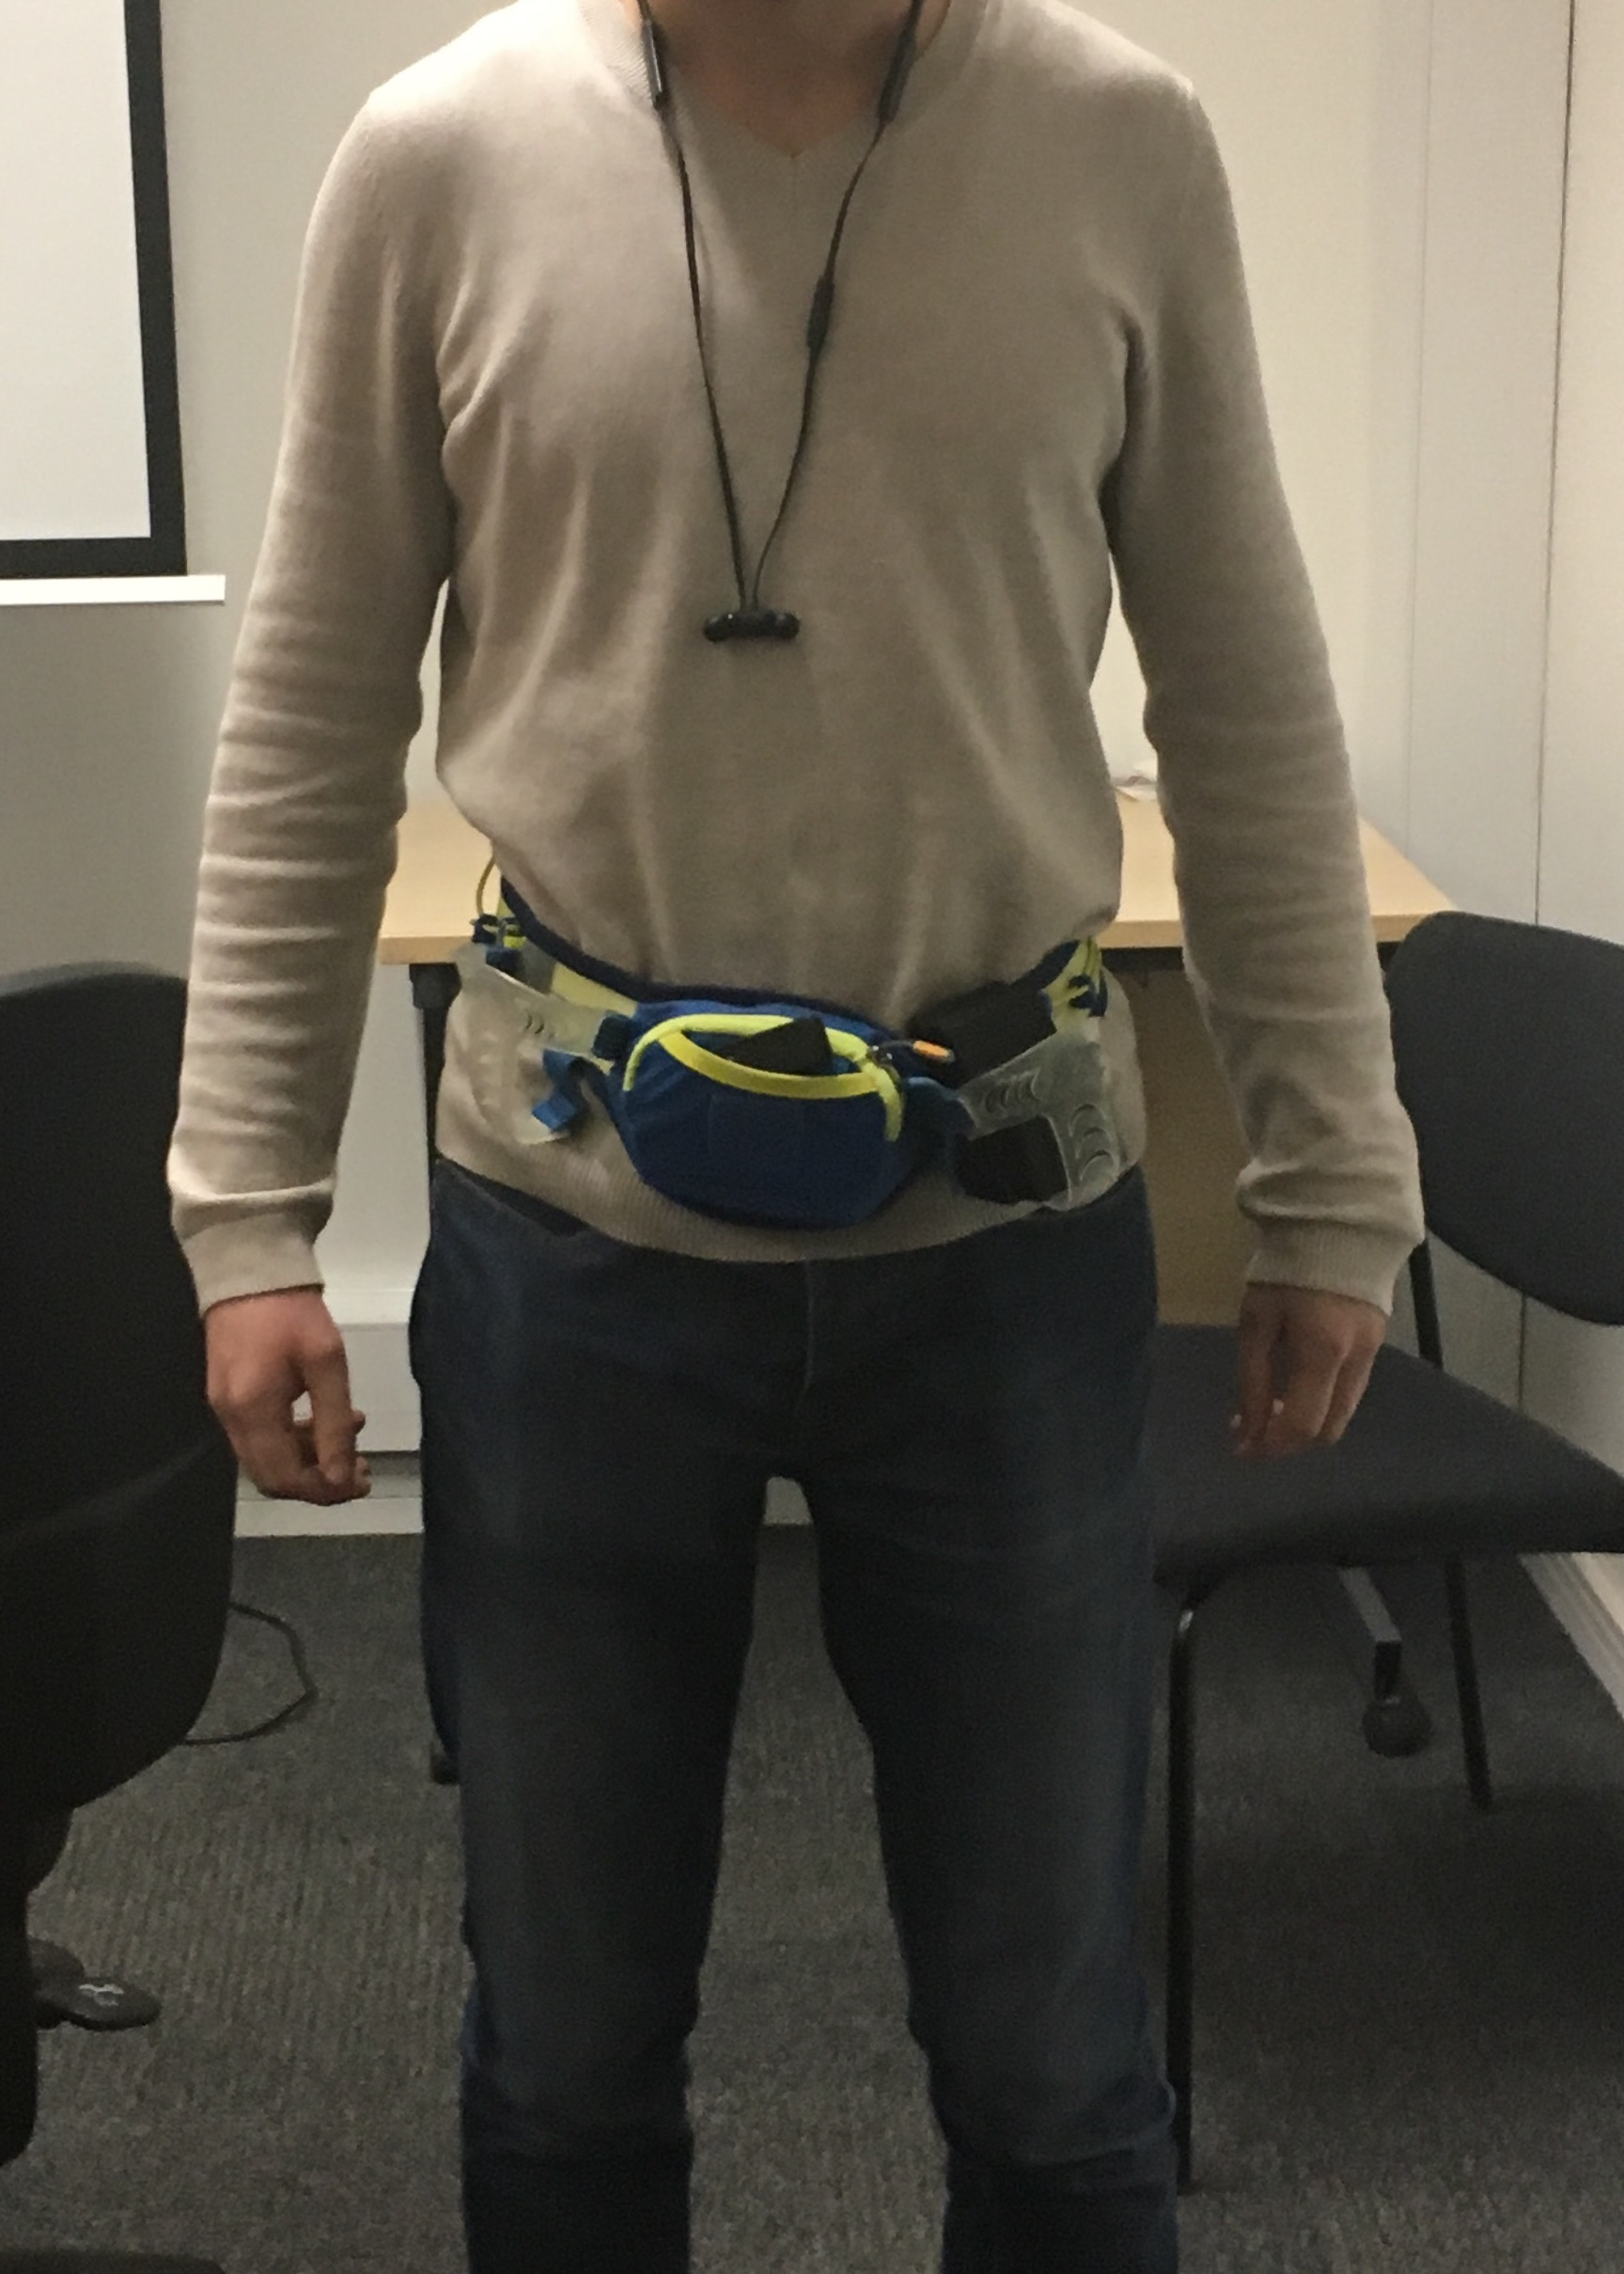
\includegraphics[width=0.6\columnwidth]{airspeck_on_me.jpg}
  \caption{This image presents the way the AirSpeck device set up with the running belt and wore during a normal data collection session.}
  \label{fig:airspeck_on_me}
\end{figure}

\chapter{Software Related Information}

\lstset{
   backgroundcolor=\color{GreenYellow!20},
   extendedchars=true,
   basicstyle=\footnotesize\ttfamily,
   showstringspaces=false,
   showspaces=false,
   numberstyle=\footnotesize,
   numbersep=8pt,
   tabsize=2,
   breaklines=true,
   showtabs=false,
   captionpos=b
}

\section{Data Visualisation Tool Setup}
\label{sec:api-setup}

The repository containing the Python code for the back-end API is located on GitHub at \url{https://github.com/MihaiVisu/hons-backend.git}. The repository is currently private and access will be made available upon request.

For development purposes, the back-end API can be installed by first installing Django and all necessary dependencies. In order to do this, a Python 3 virtual environment must be created. One way to create it is through miniconda \cite{miniconda}:

\begin{lstlisting}[language=bash, backgroundcolor=\color{lightgray!20}, basicstyle=\ttfamily\bfseries] 
	$ conda create -n <environment name> python=3.6
\end{lstlisting}

After creating the environment, all the dependencies in regard to the framework used by the API must be installed. The libraries are listed in the \texttt{requirements.txt} file and can be installed after activating the virtual environment:

\begin{lstlisting}[language=bash, backgroundcolor=\color{lightgray!20}, basicstyle=\ttfamily\bfseries] 
	$ source activate <environment name>
	$ pip install -r requirements.txt
\end{lstlisting}

Then, the server can be started by entering the main project folder and typing:

\begin{lstlisting}[language=bash, backgroundcolor=\color{lightgray!20}, basicstyle=\ttfamily\bfseries] 
	$ python manage.py runserver <port number>
\end{lstlisting}

Furthermore, the repository containing the front-end interface is available at \url{https://github.com/MihaiVisu/HonoursProject.git}. The repository is private as well and access will be made available upon request. The user must first activate the virtual environment created in the previous steps in order to be able to run it. Then, the interface server can be started by entering the code directory and running the \texttt{server.py} file.

\begin{lstlisting}[language=bash, backgroundcolor=\color{lightgray!20}, basicstyle=\ttfamily\bfseries] 
	$ source activate <environment name>
	$ python server.py
\end{lstlisting}


\section{Jupyter Notebooks Setup}

The Jupyter notebooks are located in the same repository as the front-end interface, namely at \url{https://github.com/MihaiVisu/HonoursProject.git}. In order to run and view them, the virtual environment must be activated first:

\begin{lstlisting}[language=bash, backgroundcolor=\color{lightgray!20}, basicstyle=\ttfamily\bfseries] 
	$ source activate <environment name>
	$ jupyter notebook
\end{lstlisting}


\section{Format of Input Response from the Back-end API}

\begin{lstlisting}[numbers=left, caption={This code listing represents an example of a data input in GeoJSON format, which is sent from the back-end to the front-end of the data visualization tool after performing urban environments clustering. The "label" key represents the id corresponding to either a certain urban environment or a specific mode of transport, depending on the type of request received by the API from the front-end interface.}]
{
	"type": "Feature", 
	"geometry": {
		"type": "Point",
		 "coordinates": ["-3.1892407", "55.9464430"]
	},
	"properties": {
		"id": 18352, 
		"label": "2", 
		"phone_timestamp": "20150723182228",
		"pm1": "0.8987573",
		"pm2_5": "16.0555000", 
		"pm10": "16.0555000",
		"temperature": "22.9800000", 
		"humidity": "47.4285549",
		"bin0": 6, "bin1": 0, 
		"bin2": 3, 
		"bin3": 1, 
		"bin4": 0, 
		"bin5": 2, 
		"bin6": 2, 
		"bin7": 0, 
		"bin8": 0, 
		"bin9": 0, 
		"bin10": 0, 
		"bin11": 0, 
		"bin12": 0, 
		"bin13": 0, 
		"bin14": 0, 
		"bin15": 0, 
		"total": 14, 
		"altitude": null, 
		"accuracy": null, 
		"lux_level": "0E-7", 
		"motion": "0E-7", 
	}
}
\end{lstlisting}



\section{Classifiers Menu Usage}
\label{sec:menu-usage}

The main menu varies depending on the type of classifier chosen and the validation method used. For instance, if the mixed model is chosen, then two different dropdown fields for two different sets of input attributes corresponding to each random forest classifier are displayed. Otherwise, only one field will be shown, as presented in Figure \ref{fig:classification-interface}.

\begin{figure}[h!]
  \begin{subfigure}[t]{\textwidth}
    \includegraphics[width=\textwidth]{appendix-classifiers-interface-mixed-model.png}
    \caption{Two dropdown fields corresponding to each random forest classifier are shown when the mixed model is used for classification. The user has the ability to select different sets of attributes for each classifier.}
    \label{fig:mixed-model-interface}
  \end{subfigure}
  \hfill
  \begin{subfigure}[t]{\textwidth}
    \includegraphics[width=\textwidth]{appendix-classifiers-interface-simple-classifier.png}
    \caption{One dropdown field corresponding to the classifier chosen is displayed. The user has the ability to select different attributes from the ones provided.}
    \label{fig:simple-classifier-interface}
  \end{subfigure}
  \caption{Varying attribute selection menu based on the model chosen for the modes of transport classification task.}
  \label{fig:classification-interface}
\end{figure}

For each dropdown field from the main classifiers menu, the user will be able to choose any attributes from the ones provided. A list of available attributes appears once the field is clicked, as Figure \ref{fig:attributes-interface} presents. A search by typing option is included in the functionality of the form via Semantic UI library (Figure \ref{fig:add-attributes-interface}).

\begin{figure}[h!]
  \begin{subfigure}[t]{\textwidth}
    \includegraphics[width=\textwidth]{appendix-classifiers-interface-include-bins.png}
    \caption{A quick way to include all bin counts for a certain classification or clustering task through the checkbox provided.}
    \label{fig:include-bins-interface}
  \end{subfigure}
  \hfill
  \begin{subfigure}[t]{\textwidth}
    \includegraphics[width=\textwidth]{appendix-classifiers-interface-add-attributes.png}
    \caption{An option to add new attributes for a certain classification or clustering task via searching for a specific name in the list of features provided is available.}
    \label{fig:add-attributes-interface}
  \end{subfigure}
  \caption{Functionality of dropdown fields regarding configuration of attributes to be considered for classification or clustering tasks.}
  \label{fig:attributes-interface}
\end{figure}

The user has the option to choose of whether to utilise a specific dataset for validation or not. If the checkbox is unchecked, then K-Fold cross validation will be used as a validation measure and an option specifying the number of folds to be used will be provided (Figure \ref{fig:classifiers-interface}). On the other hand, an option regarding the choice of the training dataset on which the configured model will be fitted is given, as presented in Figure \ref{fig:validation-checkbox}. As an example, Figure \ref{fig:queensferry-return-transport} presents the classification results displayed on the map interface by utilising the spatial information provided after performing modes of transport classification on the return trip from Queesnferry.

\begin{figure}[h!]
  \center
  \includegraphics[width=\columnwidth]{appendix-classifiers-interface-validation.png}
  \caption{An option of whether to utilise a certain dataset for validation is provided via the checkbox field shown in the image.}
  \label{fig:validation-checkbox}
\end{figure}

\begin{figure}[h!]
  \begin{subfigure}[t]{\textwidth}
    \includegraphics[width=\textwidth]{queensferry_transport_1.png}
    \caption{Validation data inputs labelled to corresponding modes of transport by best performing model in the first part of the route.}
    \label{fig:queensferry-return-transport-1}
  \end{subfigure}
  \hfill
  \begin{subfigure}[t]{\textwidth}
    \includegraphics[width=\textwidth]{queensferry_transport_2.png}
    \caption{Validation data inputs labelled to corresponding modes of transport by best performing model in the second part of the route.}
    \label{fig:queensferry-return-transport-2}
  \end{subfigure}
  \caption{Results obtained after utilising the best performing modes of transport classification model on the validation set of the return trip between Queensferry and Princes Street. The starting point is the bus stop in Queensferry and the ending point of the bus trip is on Princes Street, followed by a walking journey to Nicholson Street. Classification accuracy obtained was 96\%.}
  \label{fig:queensferry-return-transport}
\end{figure}

\end{appendices}

\end{document}
